% Options for packages loaded elsewhere
\PassOptionsToPackage{unicode}{hyperref}
\PassOptionsToPackage{hyphens}{url}
%
\documentclass[
]{article}
\usepackage{lmodern}
\usepackage{amssymb,amsmath}
\usepackage{ifxetex,ifluatex}
\ifnum 0\ifxetex 1\fi\ifluatex 1\fi=0 % if pdftex
  \usepackage[T1]{fontenc}
  \usepackage[utf8]{inputenc}
  \usepackage{textcomp} % provide euro and other symbols
\else % if luatex or xetex
  \usepackage{unicode-math}
  \defaultfontfeatures{Scale=MatchLowercase}
  \defaultfontfeatures[\rmfamily]{Ligatures=TeX,Scale=1}
\fi
% Use upquote if available, for straight quotes in verbatim environments
\IfFileExists{upquote.sty}{\usepackage{upquote}}{}
\IfFileExists{microtype.sty}{% use microtype if available
  \usepackage[]{microtype}
  \UseMicrotypeSet[protrusion]{basicmath} % disable protrusion for tt fonts
}{}
\makeatletter
\@ifundefined{KOMAClassName}{% if non-KOMA class
  \IfFileExists{parskip.sty}{%
    \usepackage{parskip}
  }{% else
    \setlength{\parindent}{0pt}
    \setlength{\parskip}{6pt plus 2pt minus 1pt}}
}{% if KOMA class
  \KOMAoptions{parskip=half}}
\makeatother
\usepackage{xcolor}
\IfFileExists{xurl.sty}{\usepackage{xurl}}{} % add URL line breaks if available
\IfFileExists{bookmark.sty}{\usepackage{bookmark}}{\usepackage{hyperref}}
\hypersetup{
  pdftitle={Nudging for less kludges: focusing on PMD alerts as possible kludges: open, fixed or new?},
  pdfauthor={Bruno Crotman},
  hidelinks,
  pdfcreator={LaTeX via pandoc}}
\urlstyle{same} % disable monospaced font for URLs
\usepackage[margin=1in]{geometry}
\usepackage{color}
\usepackage{fancyvrb}
\newcommand{\VerbBar}{|}
\newcommand{\VERB}{\Verb[commandchars=\\\{\}]}
\DefineVerbatimEnvironment{Highlighting}{Verbatim}{commandchars=\\\{\}}
% Add ',fontsize=\small' for more characters per line
\usepackage{framed}
\definecolor{shadecolor}{RGB}{248,248,248}
\newenvironment{Shaded}{\begin{snugshade}}{\end{snugshade}}
\newcommand{\AlertTok}[1]{\textcolor[rgb]{0.94,0.16,0.16}{#1}}
\newcommand{\AnnotationTok}[1]{\textcolor[rgb]{0.56,0.35,0.01}{\textbf{\textit{#1}}}}
\newcommand{\AttributeTok}[1]{\textcolor[rgb]{0.77,0.63,0.00}{#1}}
\newcommand{\BaseNTok}[1]{\textcolor[rgb]{0.00,0.00,0.81}{#1}}
\newcommand{\BuiltInTok}[1]{#1}
\newcommand{\CharTok}[1]{\textcolor[rgb]{0.31,0.60,0.02}{#1}}
\newcommand{\CommentTok}[1]{\textcolor[rgb]{0.56,0.35,0.01}{\textit{#1}}}
\newcommand{\CommentVarTok}[1]{\textcolor[rgb]{0.56,0.35,0.01}{\textbf{\textit{#1}}}}
\newcommand{\ConstantTok}[1]{\textcolor[rgb]{0.00,0.00,0.00}{#1}}
\newcommand{\ControlFlowTok}[1]{\textcolor[rgb]{0.13,0.29,0.53}{\textbf{#1}}}
\newcommand{\DataTypeTok}[1]{\textcolor[rgb]{0.13,0.29,0.53}{#1}}
\newcommand{\DecValTok}[1]{\textcolor[rgb]{0.00,0.00,0.81}{#1}}
\newcommand{\DocumentationTok}[1]{\textcolor[rgb]{0.56,0.35,0.01}{\textbf{\textit{#1}}}}
\newcommand{\ErrorTok}[1]{\textcolor[rgb]{0.64,0.00,0.00}{\textbf{#1}}}
\newcommand{\ExtensionTok}[1]{#1}
\newcommand{\FloatTok}[1]{\textcolor[rgb]{0.00,0.00,0.81}{#1}}
\newcommand{\FunctionTok}[1]{\textcolor[rgb]{0.00,0.00,0.00}{#1}}
\newcommand{\ImportTok}[1]{#1}
\newcommand{\InformationTok}[1]{\textcolor[rgb]{0.56,0.35,0.01}{\textbf{\textit{#1}}}}
\newcommand{\KeywordTok}[1]{\textcolor[rgb]{0.13,0.29,0.53}{\textbf{#1}}}
\newcommand{\NormalTok}[1]{#1}
\newcommand{\OperatorTok}[1]{\textcolor[rgb]{0.81,0.36,0.00}{\textbf{#1}}}
\newcommand{\OtherTok}[1]{\textcolor[rgb]{0.56,0.35,0.01}{#1}}
\newcommand{\PreprocessorTok}[1]{\textcolor[rgb]{0.56,0.35,0.01}{\textit{#1}}}
\newcommand{\RegionMarkerTok}[1]{#1}
\newcommand{\SpecialCharTok}[1]{\textcolor[rgb]{0.00,0.00,0.00}{#1}}
\newcommand{\SpecialStringTok}[1]{\textcolor[rgb]{0.31,0.60,0.02}{#1}}
\newcommand{\StringTok}[1]{\textcolor[rgb]{0.31,0.60,0.02}{#1}}
\newcommand{\VariableTok}[1]{\textcolor[rgb]{0.00,0.00,0.00}{#1}}
\newcommand{\VerbatimStringTok}[1]{\textcolor[rgb]{0.31,0.60,0.02}{#1}}
\newcommand{\WarningTok}[1]{\textcolor[rgb]{0.56,0.35,0.01}{\textbf{\textit{#1}}}}
\usepackage{graphicx,grffile}
\makeatletter
\def\maxwidth{\ifdim\Gin@nat@width>\linewidth\linewidth\else\Gin@nat@width\fi}
\def\maxheight{\ifdim\Gin@nat@height>\textheight\textheight\else\Gin@nat@height\fi}
\makeatother
% Scale images if necessary, so that they will not overflow the page
% margins by default, and it is still possible to overwrite the defaults
% using explicit options in \includegraphics[width, height, ...]{}
\setkeys{Gin}{width=\maxwidth,height=\maxheight,keepaspectratio}
% Set default figure placement to htbp
\makeatletter
\def\fps@figure{htbp}
\makeatother
\setlength{\emergencystretch}{3em} % prevent overfull lines
\providecommand{\tightlist}{%
  \setlength{\itemsep}{0pt}\setlength{\parskip}{0pt}}
\setcounter{secnumdepth}{5}
\usepackage{lscape}
\newcommand{\blandscape}{\begin{landscape}}
\newcommand{\elandscape}{\end{landscape}}
\definecolor{darkred}{RGB}{150, 40, 40}
\definecolor{darkgreen}{RGB}{30, 120, 30}
\definecolor{darkorange}{RGB}{40, 40, 160}
\newcommand{\comentario}[1]{}
\usepackage{booktabs}
\usepackage{longtable}
\usepackage{array}
\usepackage{multirow}
\usepackage{wrapfig}
\usepackage{float}
\usepackage{colortbl}
\usepackage{pdflscape}
\usepackage{tabu}
\usepackage{threeparttable}
\usepackage{threeparttablex}
\usepackage[normalem]{ulem}
\usepackage{makecell}
\usepackage{xcolor}

\title{Nudging for less kludges: focusing on PMD alerts as possible kludges:
open, fixed or new?}
\author{Bruno Crotman}
\date{}

\begin{document}
\maketitle

{
\setcounter{tocdepth}{3}
\tableofcontents
}
\small

\normalsize

\section{Introduction}\label{intro}

This document is part of a research project about software degradation
caused by careless developers' behavior and about strategies to deal
with such undesired behavior. The strategies to deal with this problem
will possibly be inspired by concepts from game theory.

We assume that software degradation can be measured by the number and
the types of kludges made by software developers in the code. One of the
goals of this project is to study how software projects evolve in terms
of number and kinds of kludges. So far, we are trying to identify
kludges by looking at alerts generated by the PMD source code analyzer.

To evaluate how the number of alerts evolve throughout the history of a
\%In Section \ref{as_whole} we present a brief summary of the broader
project that we intend to develop. In Section \ref{pmd}, we describe how
we use PMD source code analyzer in two tasks:

\%In Section \ref{as_whole} we present a brief summary of the broader
project that we intend to develop. In Section \ref{pmd}, we describe how
we use PMD source code analyzer in two tasks:

\%In Section \ref{alg}, we describe the algorithm that help to
categorize the alerts as \textbf{new}, \textbf{fixed} or \textbf{open}.

\%In Section \ref{results}, we run the algorithm on some versions of the
project ArgoUML and present some results. We compare the incidence of
new PMD alerts found by the algorithm with the incidence of new comments
that match to patterns related to Self Admitted Technical Debts.

\% ========================================================= \% \% PMD
SOURCE CODE ANALYZER \% \%
=========================================================

\section{PMD Source Code Analyzer}\label{pmd}

PMD is static source code analyzer that is commonly used to find
possible programming flaws. We use PMD for two tasks:

\begin{itemize}
\item To list the alerts that represent possible kludges. PMD receives a source code as input and generates a list of bad programming practices 
contained in the code, i.e., the alerts. The process we follow to generate the alerts using PMD source code analyzer is discussed in Section \ref{history};

\item To create an Abstract Syntax Tree (AST) from a source code with selected nodes. This will help us in the algorithm described in Section \ref{alg}. The creation of the AST using PMD is described in Section \ref{ast}.
\end{itemize}

PMD traverses the AST of a source code searching for violations of rules
which are configured by the user. PMD comes with a default rule set for
the Java programming language. The default rule set finds common
programming flaws such as unused variables, empty catch blocks,
unnecessary object creation, and so forth. It is possible to configure a
different set of rules by creating a custom XML file. In Figure
\ref{simple_code}, we can see an example of a simple code and the alerts
that were generated by the default rule set of PMD alerts tool.

\small

\normalsize

\small

\begin{Shaded}
\begin{Highlighting}[]
\CommentTok{/*  1-                                   */}\KeywordTok{package}\ImportTok{ pack_x;}
\CommentTok{/*  2-                                   */}  
\CommentTok{/*  3-                                   */}\KeywordTok{import}\ImportTok{ importX.function;}
\CommentTok{/*  4-                                   */}
\CommentTok{/*  5-                                   */}\KeywordTok{class}\NormalTok{ ClassX }\KeywordTok{extends}\NormalTok{ ClassY }\KeywordTok{implements}\NormalTok{ InterfX \{}
\CommentTok{/*  6-                                   */}    \KeywordTok{private} \DataTypeTok{long}\NormalTok{ fieldX;}
\CommentTok{/*  7-                                   */}    
\CommentTok{/*  8-                                   */}    \FunctionTok{ClassX}\NormalTok{(}\DataTypeTok{int}\NormalTok{ paramX, }\DataTypeTok{double}\NormalTok{ paramY) \{      }
\CommentTok{/*  9-                                   */}        \DataTypeTok{int}\NormalTok{ varX = }\FunctionTok{function}\NormalTok{(paramX, paramY);     }
\CommentTok{/* 10-                                   */}        \KeywordTok{if}\NormalTok{ (varX == }\DecValTok{0}\NormalTok{)}
\CommentTok{/* 11-ControlStatementBraces             */}            \KeywordTok{this}\NormalTok{.}\FunctionTok{fieldX}\NormalTok{ = }\DecValTok{1}\NormalTok{;}
\CommentTok{/* 12-                                   */}        \KeywordTok{else}\NormalTok{\{}
\CommentTok{/* 13-                                   */}            \KeywordTok{this}\NormalTok{.}\FunctionTok{fieldX}\NormalTok{ = }\DecValTok{0}\NormalTok{;}
\CommentTok{/* 14-                                   */}\NormalTok{     \}}
\CommentTok{/* 15-                                   */}\NormalTok{    \}}
\CommentTok{/* 16-                                   */}    \AttributeTok{@Override}
\CommentTok{/* 17-                                   */}    \KeywordTok{public} \DataTypeTok{int} \FunctionTok{methodX}\NormalTok{(}\DataTypeTok{int}\NormalTok{ paramW, }\BuiltInTok{Boolean}\NormalTok{ paramZ)}
\CommentTok{/* 18-                                   */}\NormalTok{    \{}
\CommentTok{/* 19-                                   */}        \KeywordTok{if}\NormalTok{ (paramZ)}
\CommentTok{/* 20-ControlStatementBraces             */}\NormalTok{            fieldX = paramW;}
\CommentTok{/* 21-                                   */}        \KeywordTok{else}\NormalTok{\{}
\CommentTok{/* 22-                                   */}\NormalTok{            fieldX = }\DecValTok{0}\NormalTok{;}
\CommentTok{/* 23-                                   */}\NormalTok{     \}}
\CommentTok{/* 24-                                   */}        \KeywordTok{return}\NormalTok{ paramW + }\KeywordTok{this}\NormalTok{.}\FunctionTok{fieldX}\NormalTok{;}
\CommentTok{/* 25-                                   */}\NormalTok{     \}}
\CommentTok{/* 26-                                   */}\NormalTok{\}  }
\end{Highlighting}
\end{Shaded}

\normalsize

\begin{figure}
\centering

\includegraphics{figures/fake.png}
\caption{Simple code with its alerts \label{simple_code}}
\end{figure}

\subsection{Using PMD to capture the history of alerts}\label{history}

To evaluate how the number of alerts evolved throughout the history of a
software project, we must be able to analyze two different versions of a
source code (an old and a new version) and categorize each alert
contained in the new version as either \textbf{new}, \textbf{fixed} or
\textbf{open}.

We define a PMD alert generated for the old version as either
\textbf{open} or \textbf{fixed} in the new version. An \textbf{open}
alert remains in the new version of the code. A \textbf{fixed} alert
does not exist in the new version.

A PMD alert generated for the new version is either \textbf{open} or
\textbf{new}. An \textbf{open} alert indicates that the same alert was
identified in the old version of the source code. A \textbf{new} alert
implies that the same alert cannot be identified in the old version.

The intersection between \textbf{fixed} alerts, \textbf{new} alerts and
\textbf{open} alerts is empty. The alerts identified as \textbf{open}
are equivalent in both new and old versions. To decide whether an alert
is \textbf{open}, \textbf{fixed} or \textbf{new}, one has to identify if
an alert in the old version is equivalent to an alert in the new
version. This document describes the algorithm we propose to make this
classification. At this point we use the default rule set to generate
the alerts.

\subsection{Using PMD to generate an Abstract Syntax Tree}\label{ast}

The AST is used to understand the location of an alert in a version of a
code. We use this information in the algorithm described in Section
\ref{alg}.

PMD traverses the source code visiting many different kinds of elements
comprising the AST. If we build our own rules, aimed to capture only
some kinds of elements, we will generate list of ``alerts'' that will
contain all the elements of the chosen kinds contained in the AST.

\section{PMD Source Code Analyzer}\label{pmd}

PMD is static source code analyzer that is commonly used to find
possible programming flaws. In this work we use PMD for two tasks: to
generate alerts that we interpret as clues about kludges and to create
an AST from the source code with selected kinds of node.

\subsection{Using PMD Source Code Analyzer to generate alerts}\label{pmd_alerts}

PMD traverses the AST of a source code searching for violations of rules
which are configured by the user. PMD comes with a default rule set for
Java language. The default rule set finds common programming flaws like
unused variables, empty catch blocks, unnecessary object creation, and
so forth. It´s possible to configure a different set of rules creating a
custom XML file. At this point we use the default rule set to generate
the alerts that we interpret as kludges and try to categorize by the
algorithm described in Section \ref{alg}

\newpage

In Figure \ref{simple_code}, we can see an example of a simple code and
the alerts that were generated by the default rule set of PMD alerts
tool.

\subsection{Using PMD to generate an Abstract Syntax Tree }\label{ast}

The AST is used, in conjunction with the relation between the lines we
will see in Section \ref{map}, to understand the location of an alert in
a version of a code. We use this information in the algorithm described
in Section \ref{alg2}. The tree helps us in making matches between the
old and the new versions that are not exact. Rather then betting on a
match that depends solely on the location of the node where the alert
is, we can get the information that the alerts are not in the same line
but belong to methods that are in the same line, for instance.

We can see that the tool traverses the source code visiting many
different kinds of elements. If we build our own simple rules, aimed
only to capture some kinds of elements, we will generate list of
``alerts'' that will contain \_all\_re the elements of the chosen kinds
contained in the AST.

\newpage

We do not use all the types of nodes recognized by PMD Alert to generate
the AST because there are many kinds of nodes and some of them are
redundant for our purposes. If we used all the kinds of nodes, we would
end up with a tree that would not add value to our analysis but would
add compelexity to our algorithm. The kinds of elements that were
selected are the following ones:

\begin{itemize}

\item \textbf{Annotation}: a syntatic metadata added to a source code;

\item \textbf{Block}: a block of statements enclosed by braces;

\item \textbf{ClassOrInterfaceBody}: the body of an interface or a class, excluding the declaration;

\item \textbf{ClassOrInterfaceDeclaration}: class or interface, including the declaration and the body;

\item \textbf{ClassOrInterfaceType}: declaration of a type;

\item \textbf{CompilationUnit}: the root of an AST tree;

\item \textbf{ConstructorDecaration}: class or interface, including the declaration and the body;

\item \textbf{ExtendsList}: list of extensions of a class;

\item \textbf{FieldDeclaration}: field declaration, including the type, name and possible assignment;

\item \textbf{FormalParameter}: a parameter of a method or constructor;

\item \textbf{FormalParameters}:  list of formal parameters of a method or constructor;

\item \textbf{IfStatement}: an if statements including its blocks and condition;

\item \textbf{ImplementsList}: list of implementations of an interface;

\item \textbf{Import}: a package imported;

\item \textbf{Method}: a method, including body and declaration;

\item \textbf{Name}: a named value, like a variable, a class or a package referenced in the code.

\item \textbf{Package}: the indication of the package to which the compilation unit belongs;

\item \textbf{Statement}: any statement, like an if statement or an assignment;

\item \textbf{TypeDeclaration}: any type declaration;

\item \textbf{VariableId}: the name of a variable in a variable declaration.
\end{itemize}

We follow three steps to recreate the AST:

\begin{enumerate}
\def\labelenumi{\arabic{enumi}.}
\item
  Link each element \(a\) to the set of elements \(X\) that are fully
  contained between the begin line / begin column and end line / end
  column of element \(a\). We can construct a directed graph in which
  the elements are the nodes and the links described are the edges. This
  is not a tree yet, because each node will have edges directed to all
  its descendants and not only its children in the AST.

\item
  Sort the nodes in the decreasing order of its number of children. The
  objective is to establish that, in a search through this graph, the
  first child chosen will be the one that is a child in the AST, and not
  only a descendant.

\item
  Proceed a deep-first search starting from the compilation unit node.
\end{enumerate}

\% \% MARCIO: eu não entendi o objetivo do algoritmo acima. Você quer
montar a AST somente \% com os tipos de nós que listou acima? Por quê?
Justifique. Depois disso, quer recriar \% o código-fonte a partir desta
AST parcial? Porque precisa disso? \%

\% \% BRUNO: A quantidade de tipos de nós é gigantesca. A árvore fica
gigantesca e muito redundante. A ideia é permitir matches que não sejam
puramente baseados \% na localização das linhas. Expliquei no texto. Às
vezes pode não bater exatamente a localização, mas o nó método pai pode
bater, portanto, podemos \% considerar que os nós estão no mesmo método
e se eles forem de mesmo tipo, com o mesmo alerta, debaixo do mesmo
método\ldots{} se tiver muita evidência de que \% é a mesma coisa,
podemos considerar que é. Aquela história: tem focinho de porco, orelha
de porco, pé de porco. É porco? Só não sei como escrever isso \% para um
inglês\ldots{} \% \%

\section{The research project}
\label{as_whole}

The aim of this section is to keep track of some discussions related to
the project in a broader sense.

\subsection{Research project stages}
\label{research-stages}

These are the planned steps of the project:

\begin{itemize}
\item
  Confirm the assumption that the frequency of PMD Alerts is an accurate
  measure of the prevalence of kludges;
\item
  Confirm the assumption that kludges harm software development;
\item
  Confirm the assumption that there is a game in which, in Nash
  equilibrium, a developer chooses a strategy in which he gets personal
  benefits while causing harm to the project, by making kludges;
\item
  If all these assumptions are true, use mechanism design to devise how
  we can change the environment in a way that developers do not choose
  to make so much kludge, increasing the quality of the project in the
  long run.
\item
  Implement this mechanism building a plugin for a prominent CI tool,
  such as Travis or Jenkins or GitLab.
\end{itemize}

\subsection{Kludge definition}\label{kludge definition}

A kludge is code that

\begin{enumerate}
\def\labelenumi{\arabic{enumi}.}
\tightlist
\item
  Partially fixes a bug or partially implements a feature.
\end{enumerate}

The term partial can be understood as in \textit{partial functions}. A
partial function is undefined for some elements in the formal domain.
For instance, the square root function restricted to the integers:
\(f(25)\) is defined, but \(f(26)\) is undefined. In terms of features,
we can think about a developer calculating the point on which two lines
cross and neglecting the case of parallel lines

\begin{enumerate}
\def\labelenumi{\arabic{enumi}.}
\setcounter{enumi}{1}
\tightlist
\item
  The developer knows that the code is only a partial solution, with
  high probability.
\end{enumerate}

It is necessary to study technical debt papers to enrich the conceptual
background.

\subsection{Research questions}

\noindent
\textbf{RQ: Is the frequency of PMD Alerts an accurate measure of the prevalence of kludges?}
\%\label{PMD_Kludge}

We have to identify events with an intense introduction of PMD Alert. To
do this we have to be able to categorize open, new and fixed PMD Alerts.

For each pair of an old and a new version of a source code, we can
measure the intensity of possible kludge introduction occurred. This
evidence of possible kludge introduction must be normalized by the size
of the change in source code between the two versions. The measure may
follow a formula like:

\% \% MARCIO: você pode medir o ``número de alertas''. No texto, você
está trocando este \% termo por kludge, mas esta relação é justamente o
que você quer provar. \%

\% \% BRUNO: Sim, agora eu chamei de possible kludges. \%

\[ \frac{\#NewAlerts - \#FixedAlerts}{Change}    \]

or

\[ \frac{\#NewAlerts - \#FixedAlerts}{\#NewAlerts + \#FixedAlerts}    \]

With these events identified, including their location in the code and
their position in the time line of commits, we can measure the
correlation of these events with some other evidence of kludge. In
Section \ref{results} we calulate these metrics for

\% \% MARCIO: o que seria ``their moment''? Uma versão em que foram
introduzidos? \% se você está preocupado com a introdução de issues,
porque está tratando \% os issues resolvidos (no numerador) nas fórmulas
acima? \%

\% \%BRUNO: Na primerira fórmula eu vou usar uma medida baseada no
número de linhas, na segunda realmente eu uso o número total de alertas.
É uma proporção de \% de quantos são os novos alertas em relação ao
núymero total de alertas. O número total de alertas fechados e abertos
serviria como ``tamanho da mudança''. \% É ruim? \% \%

An evidence could be churns around the location of the event in
subsequent commits. And this would be related with the statement 1 of
the definition of kludge in Section \ref{roadmap}.

Other possible evidence could be survey and bag of words mining of
issue, mailing lists, and commit messages showing evidence of kludge
game. This could be related more with the Statement 2 of the definition
of kludge in Section \ref{roadmap}.

\vspace{32px}

\textbf{RQ: Do kludges harm software development?} \label{kludge_harm}

We need some way to measure degradation after a heavy introduction of
kludges. A drop in the popularity may not be a proper evidence. The
increment in the number of issues and bug fixed nor necessarily
represent a degradation. Churn could be used here.

\% ========================================================= \% \%
ALGORITHMS \% \%
=========================================================

\section{Algorithm to categorize alerts}\label{alg}

This Section discusses the algorithm to categorize alerts, which uses
the AST to create features that help to infer if two alerts in different
versions must be considered the same. This algorithm does not return a
single categorical answer for each alert (new, open or fixed), but
features that must be evaluated by some heuristic or possibly a
statistical learning tool.

In Section \ref{source_used} the source code used in this description is
shown. Section \ref{map} describes how the source code lines are mapped.
In the Section \ref{feature_creation}, we show how the features are
created. Even though it is not possible to be sure if a pair alerts in
different versions are same alert, we think that these features can
provide some clues. The heuristic we used for this work is described in
Section \ref{heuristic}.

\% \% MARCIO: retorna features? o que são estas features? \%

\% \% BRUNO: o pessoal de aprendizado estatístico que chama de feature
cada tipo de dado usado como entrada nos modelos deles. Tem até uma área
de feature \% engineering, que serve pra gerar, a partir dos dados
brutos, esses dados de entrada que facilitam a vida do modelo. Por
exemplo, ao invés de enfiar num \% modelo uma imagem de um exame, vc
pode fazer primeiro um tratamento que extrai o diâmetro médio das
células que ele encontra na imagem. Seria o paralelo \% de em vez de
meter no nosso modelo (que no caso é uma heurística) o código-fonte
todo, a gente meter essas features pra que seja mais fácil definir a \%
classificação do alerta. Vc acha que vale a pena eu escrever essas
coisas no texto?

\newpage

\begin{landscape}

\subsection{Source code used}\label{source_used}

In this Section, we will consider the old and new version of a source
code as presented in Figure \ref{old_simple_code} and the new version in
Figure \ref{new_simple_code}. In the new version, the alert generated in
the line 11 of the old version was fixed.

\scriptsize

\begin{Shaded}
\begin{Highlighting}[]
\CommentTok{/*  1-                 */}\KeywordTok{package}\ImportTok{ pack_x;                                                /*  1-                 */package pack_x;}                                                
\CommentTok{/*  2-                 */}                                                               \CommentTok{/*  2-                 */}                                                               
\CommentTok{/*  3-                 */}\KeywordTok{import}\ImportTok{ importX.function;                                       /*  3-                 */import importX.function;}                                       
\CommentTok{/*  4-                 */}                                                               \CommentTok{/*  4-                 */}                                                               
\CommentTok{/*  5-                 */}\KeywordTok{class}\NormalTok{ ClassX }\KeywordTok{extends}\NormalTok{ ClassY }\KeywordTok{implements}\NormalTok{ InterfX \{               }\CommentTok{/*  5-                 */}\KeywordTok{class}\NormalTok{ ClassX }\KeywordTok{extends}\NormalTok{ ClassY }\KeywordTok{implements}\NormalTok{ InterfX \{               }
\CommentTok{/*  6-                 */}    \KeywordTok{private} \DataTypeTok{long}\NormalTok{ fieldX;                                       }\CommentTok{/*  6-                 */}    \KeywordTok{private} \DataTypeTok{long}\NormalTok{ fieldX;                                       }
\CommentTok{/*  7-                 */}                                                               \CommentTok{/*  7-                 */}                                                               
\CommentTok{/*  8-                 */}    \FunctionTok{ClassX}\NormalTok{(}\DataTypeTok{int}\NormalTok{ paramX, }\DataTypeTok{double}\NormalTok{ paramY) \{                                }\CommentTok{/*  8-                 */}    \FunctionTok{ClassX}\NormalTok{(}\DataTypeTok{int}\NormalTok{ paramX, }\DataTypeTok{double}\NormalTok{ paramY) \{                                }
\CommentTok{/*  9-                 */}        \DataTypeTok{int}\NormalTok{ varX = }\FunctionTok{function}\NormalTok{(paramX, paramY);                          }\CommentTok{/*  9-                 */}        \DataTypeTok{int}\NormalTok{ varX = }\FunctionTok{function}\NormalTok{(paramX, paramY);                           }
\CommentTok{/* 10-                 */}        \KeywordTok{if}\NormalTok{ (varX == }\DecValTok{0}\NormalTok{)                                         }\CommentTok{/* 10-                 */}        \KeywordTok{if}\NormalTok{ (varX == }\DecValTok{0}\NormalTok{)                                         }
\CommentTok{/*   -                 *//*XXXXXXXXXXXXXXXXXXXXXXXXXXXXXXXXXXXXXX*/}                     \CommentTok{/* 11-                 */}\NormalTok{        \{                                                      }
\CommentTok{/* 11-ControlStateme   */}            \KeywordTok{this}\NormalTok{.}\FunctionTok{fieldX}\NormalTok{ = }\DecValTok{1}\NormalTok{;                                   }\CommentTok{/* 12-                 */}            \KeywordTok{this}\NormalTok{.}\FunctionTok{fieldX}\NormalTok{ = }\DecValTok{1}\NormalTok{;                                   }
\CommentTok{/*   -                 *//*XXXXXXXXXXXXXXXXXXXXXXXXXXXXXXXXXXXXXX*/}                     \CommentTok{/* 13-                 */}\NormalTok{        \}                                                                }
\CommentTok{/* 12-                 */}        \KeywordTok{else}\NormalTok{\{                                                  }\CommentTok{/* 14-                 */}        \KeywordTok{else}\NormalTok{\{                                                  }
\CommentTok{/* 13-                 */}            \KeywordTok{this}\NormalTok{.}\FunctionTok{fieldX}\NormalTok{ = }\DecValTok{0}\NormalTok{;                                   }\CommentTok{/* 15-                 */}            \KeywordTok{this}\NormalTok{.}\FunctionTok{fieldX}\NormalTok{ = }\DecValTok{0}\NormalTok{;                                   }
\CommentTok{/* 14-                 */}\NormalTok{       \}                                                              }\CommentTok{/* 16-                 */}\NormalTok{        \}                                                              }
\CommentTok{/* 15-                 */}\NormalTok{    \}                                                          }\CommentTok{/* 17-                 */}\NormalTok{    \}                                                          }
\CommentTok{/* 16-                 */}    \AttributeTok{@Override}                                                  \CommentTok{/* 18-                 */}    \AttributeTok{@Override}                                                  
\CommentTok{/* 17-                 */}    \KeywordTok{public} \DataTypeTok{int} \FunctionTok{methodX}\NormalTok{(}\DataTypeTok{int}\NormalTok{ paramW, }\BuiltInTok{Boolean}\NormalTok{ paramZ)             }\CommentTok{/* 19-                 */}    \KeywordTok{public} \DataTypeTok{int} \FunctionTok{methodX}\NormalTok{(}\DataTypeTok{int}\NormalTok{ paramW, }\BuiltInTok{Boolean}\NormalTok{ paramZ)             }
\CommentTok{/* 18-                 */}\NormalTok{    \{                                                          }\CommentTok{/* 20-                 */}\NormalTok{    \{                                                          }
\CommentTok{/* 19-                 */}        \KeywordTok{if}\NormalTok{ (paramZ)                                            }\CommentTok{/* 21-                 */}        \KeywordTok{if}\NormalTok{ (paramZ)                                            }
\CommentTok{/* 20-ControlStateme   */}\NormalTok{            fieldX = paramW;                                   }\CommentTok{/* 22-ControlStateme   */}\NormalTok{            fieldX = paramW;                                   }
\CommentTok{/* 21-                 */}        \KeywordTok{else}\NormalTok{\{                                                  }\CommentTok{/* 23-                 */}        \KeywordTok{else}\NormalTok{\{                                                  }
\CommentTok{/* 22-                 */}\NormalTok{            fieldX = }\DecValTok{0}\NormalTok{;                                        }\CommentTok{/* 24-                 */}\NormalTok{            fieldX = }\DecValTok{0}\NormalTok{;                                        }
\CommentTok{/* 23-                 */}\NormalTok{       \}                                                              }\CommentTok{/* 25-                 */}\NormalTok{        \}                                                              }
\CommentTok{/* 24-                 */}        \KeywordTok{return}\NormalTok{ paramW + }\KeywordTok{this}\NormalTok{.}\FunctionTok{fieldX}\NormalTok{;                           }\CommentTok{/* 26-                 */}        \KeywordTok{return}\NormalTok{ paramW + }\KeywordTok{this}\NormalTok{.}\FunctionTok{fieldX}\NormalTok{;                           }
\CommentTok{/* 25-                 */}\NormalTok{     \}                                                         }\CommentTok{/* 27-                 */}\NormalTok{     \}                                                         }
\CommentTok{/* 26-                 */}\NormalTok{\}                                                              }\CommentTok{/* 28-                 */}\NormalTok{\}                                                              }
\end{Highlighting}
\end{Shaded}

\normalsize

\begin{figure}
\centering

\includegraphics{figures/fake.png}
\caption{Source code used in the description of the algorithm}
\end{figure}

\end{landscape}

\newpage

\subsection{Using information from git diff, create a relation between the lines}\label{map}

For each difference stated in the output (the sections of the diff file
starting with ``@@''), there is an indication of the number of lines
removed from the old version and the number of lines added to the new
one. The line in which the lines are removed from the old version and
the line at which the lines are added is indicated, too.\\
By using this information we create a relation between the lines of the
old version and the equivalent lines in the new version. For the new and
old versions presented in Section \ref{codes}, the relation is shown in
Table \ref{table_map}.

\small

\begin{table}

\caption{\label{tab:showing map}Relation between lines of the old version and lines of the new version\label{table_map}}
\centering
\resizebox{\linewidth}{!}{
\begin{tabular}[t]{l|l|l|l|l|l|l|l|l|l|l|l|l|l|l}
\hline
1 & 2 & 3- & -8 & 9 & 10 & \textcolor{white}{7} & 11 & \textcolor{white}{9} & 12 & 13 & 14- & -24 & 25 & 26\\
\hline
1 & 2 & 3- & -8 & 9 & 10 & 11 & 12 & 13 & 14 & 15 & 16- & -26 & 27 & 28\\
\hline
\end{tabular}}
\end{table}

\normalsize

\subsection{Feature engineering} \label{feature_creation}

In Figure \ref{AST_compare_id_alerts} we can see the ASTs for the old
and the new versions. We can see the kind of nodes and the PMD alert if
there is one. In this figures, the numbers in the nodes are meaningless
and are presented only for reference.

\small

\begin{figure}[H]
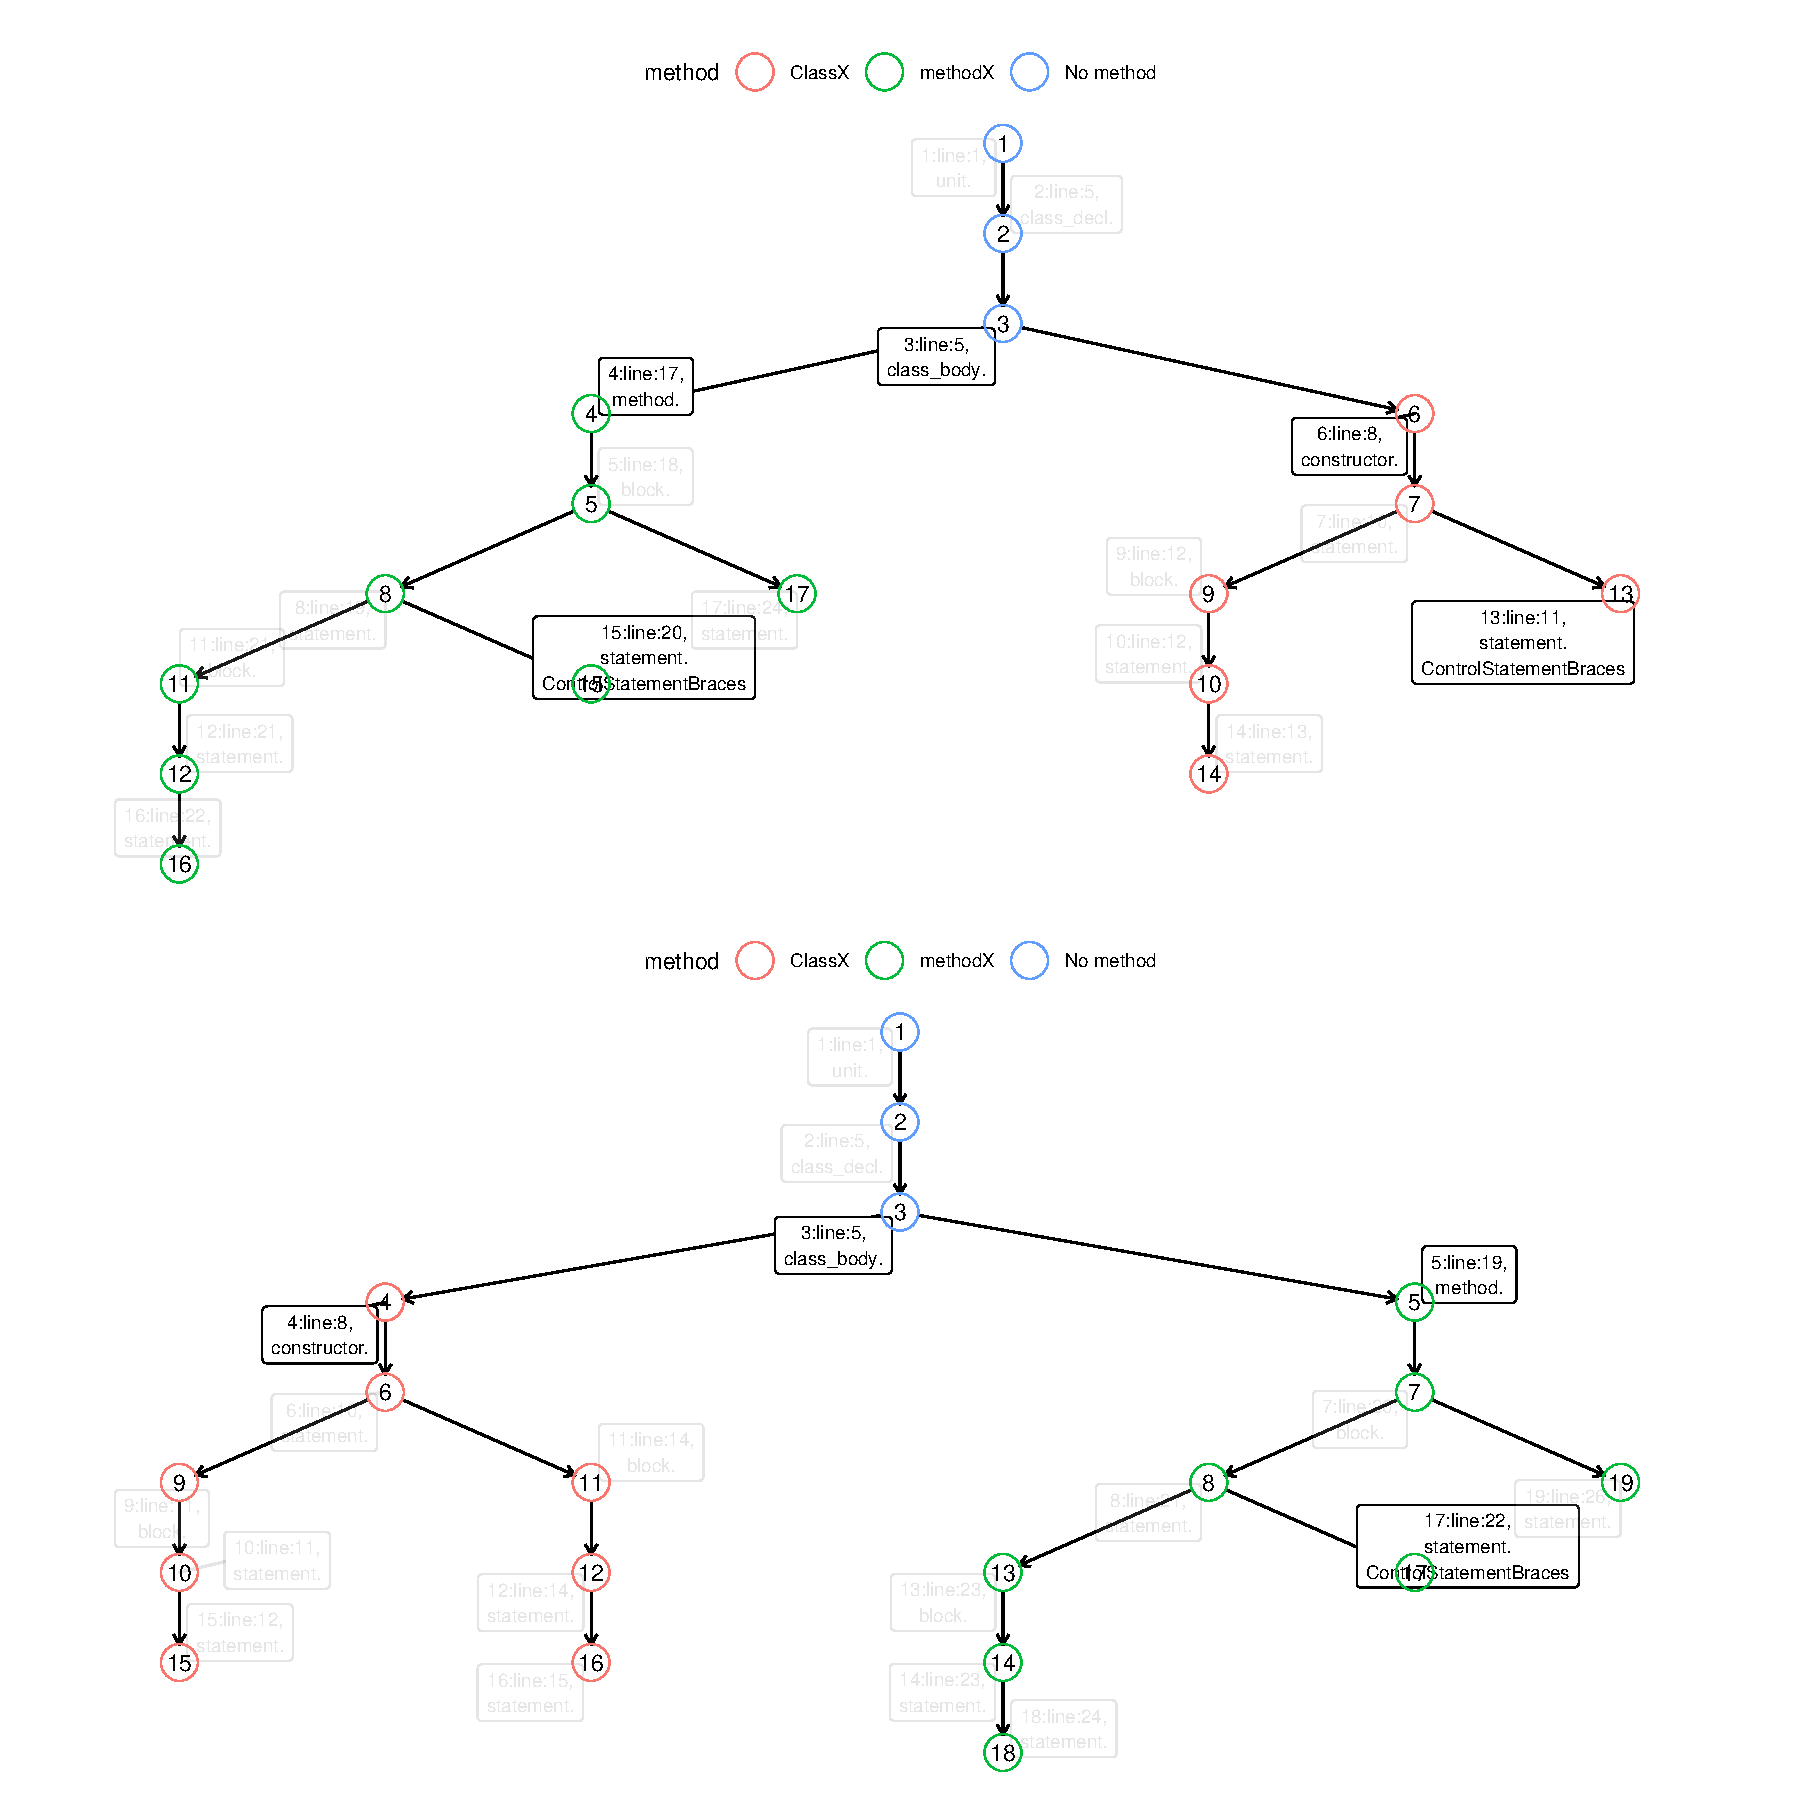
\includegraphics[width=1\linewidth]{report_files/figure-latex/unnamed-chunk-2-1} \caption{Abstract Syntax Trees. New and old versions, with alerts \label{AST_compare_id_alerts}}\label{fig:unnamed-chunk-2}
\end{figure}

\normalsize

\begin{itemize}
\item
  Considering the relation between the lines of the two versions constructed as we saw in Section \ref{map}, the nodes in both trees begin and end in related lines;

\item
  The nodes are of the same kind.
\end{itemize}

\small

\begin{figure}[H]
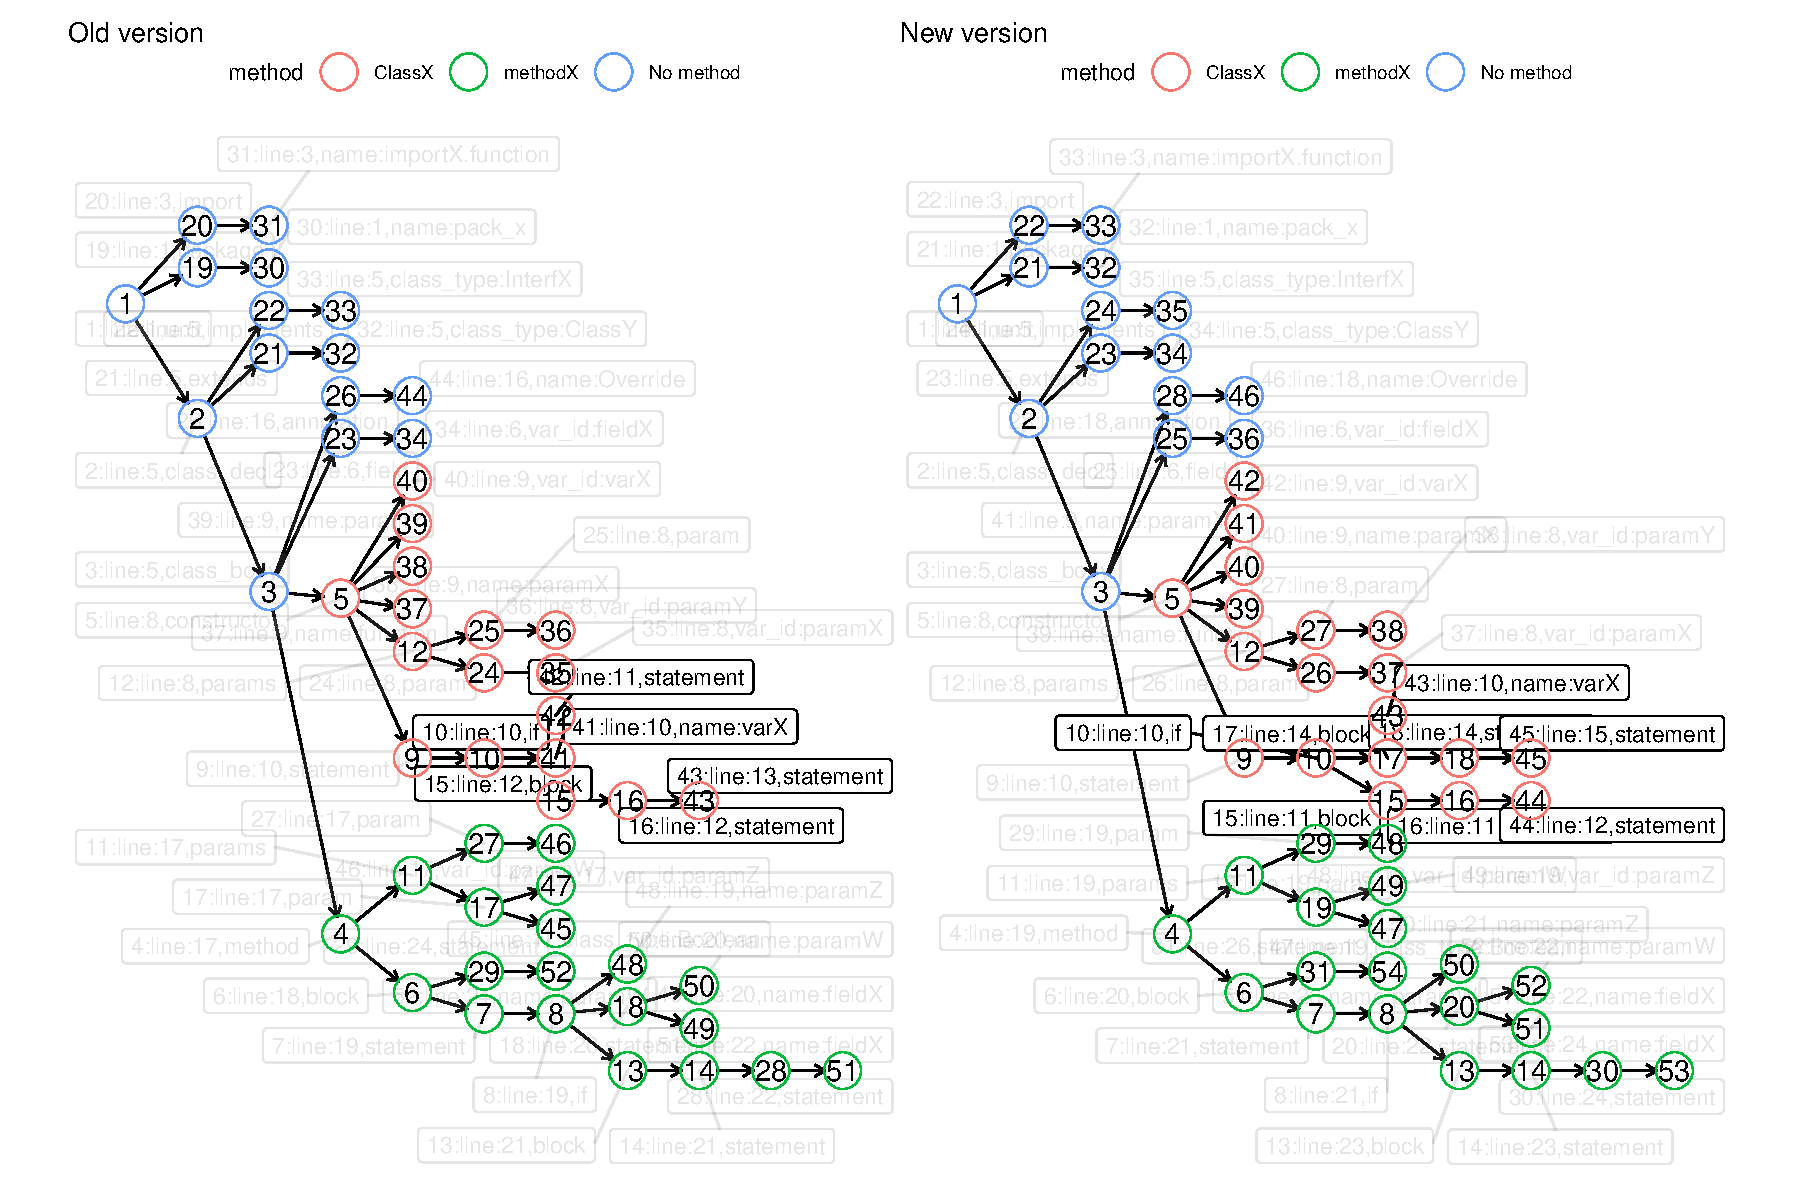
\includegraphics[width=1\linewidth]{report_files/figure-latex/unnamed-chunk-3-1} \caption{Abstract Syntax Tree. Nodes with the same number are equivalent \label{AST_with_alerts}}\label{fig:unnamed-chunk-3}
\end{figure}

\normalsize

The path between the alert and the root of the AST can be seen in
\ref{AST_alert_1}. Comparing the path of different alerts is possible to
determine if the nodes belong to the same method, for instance.

\small

\begin{figure}[H]
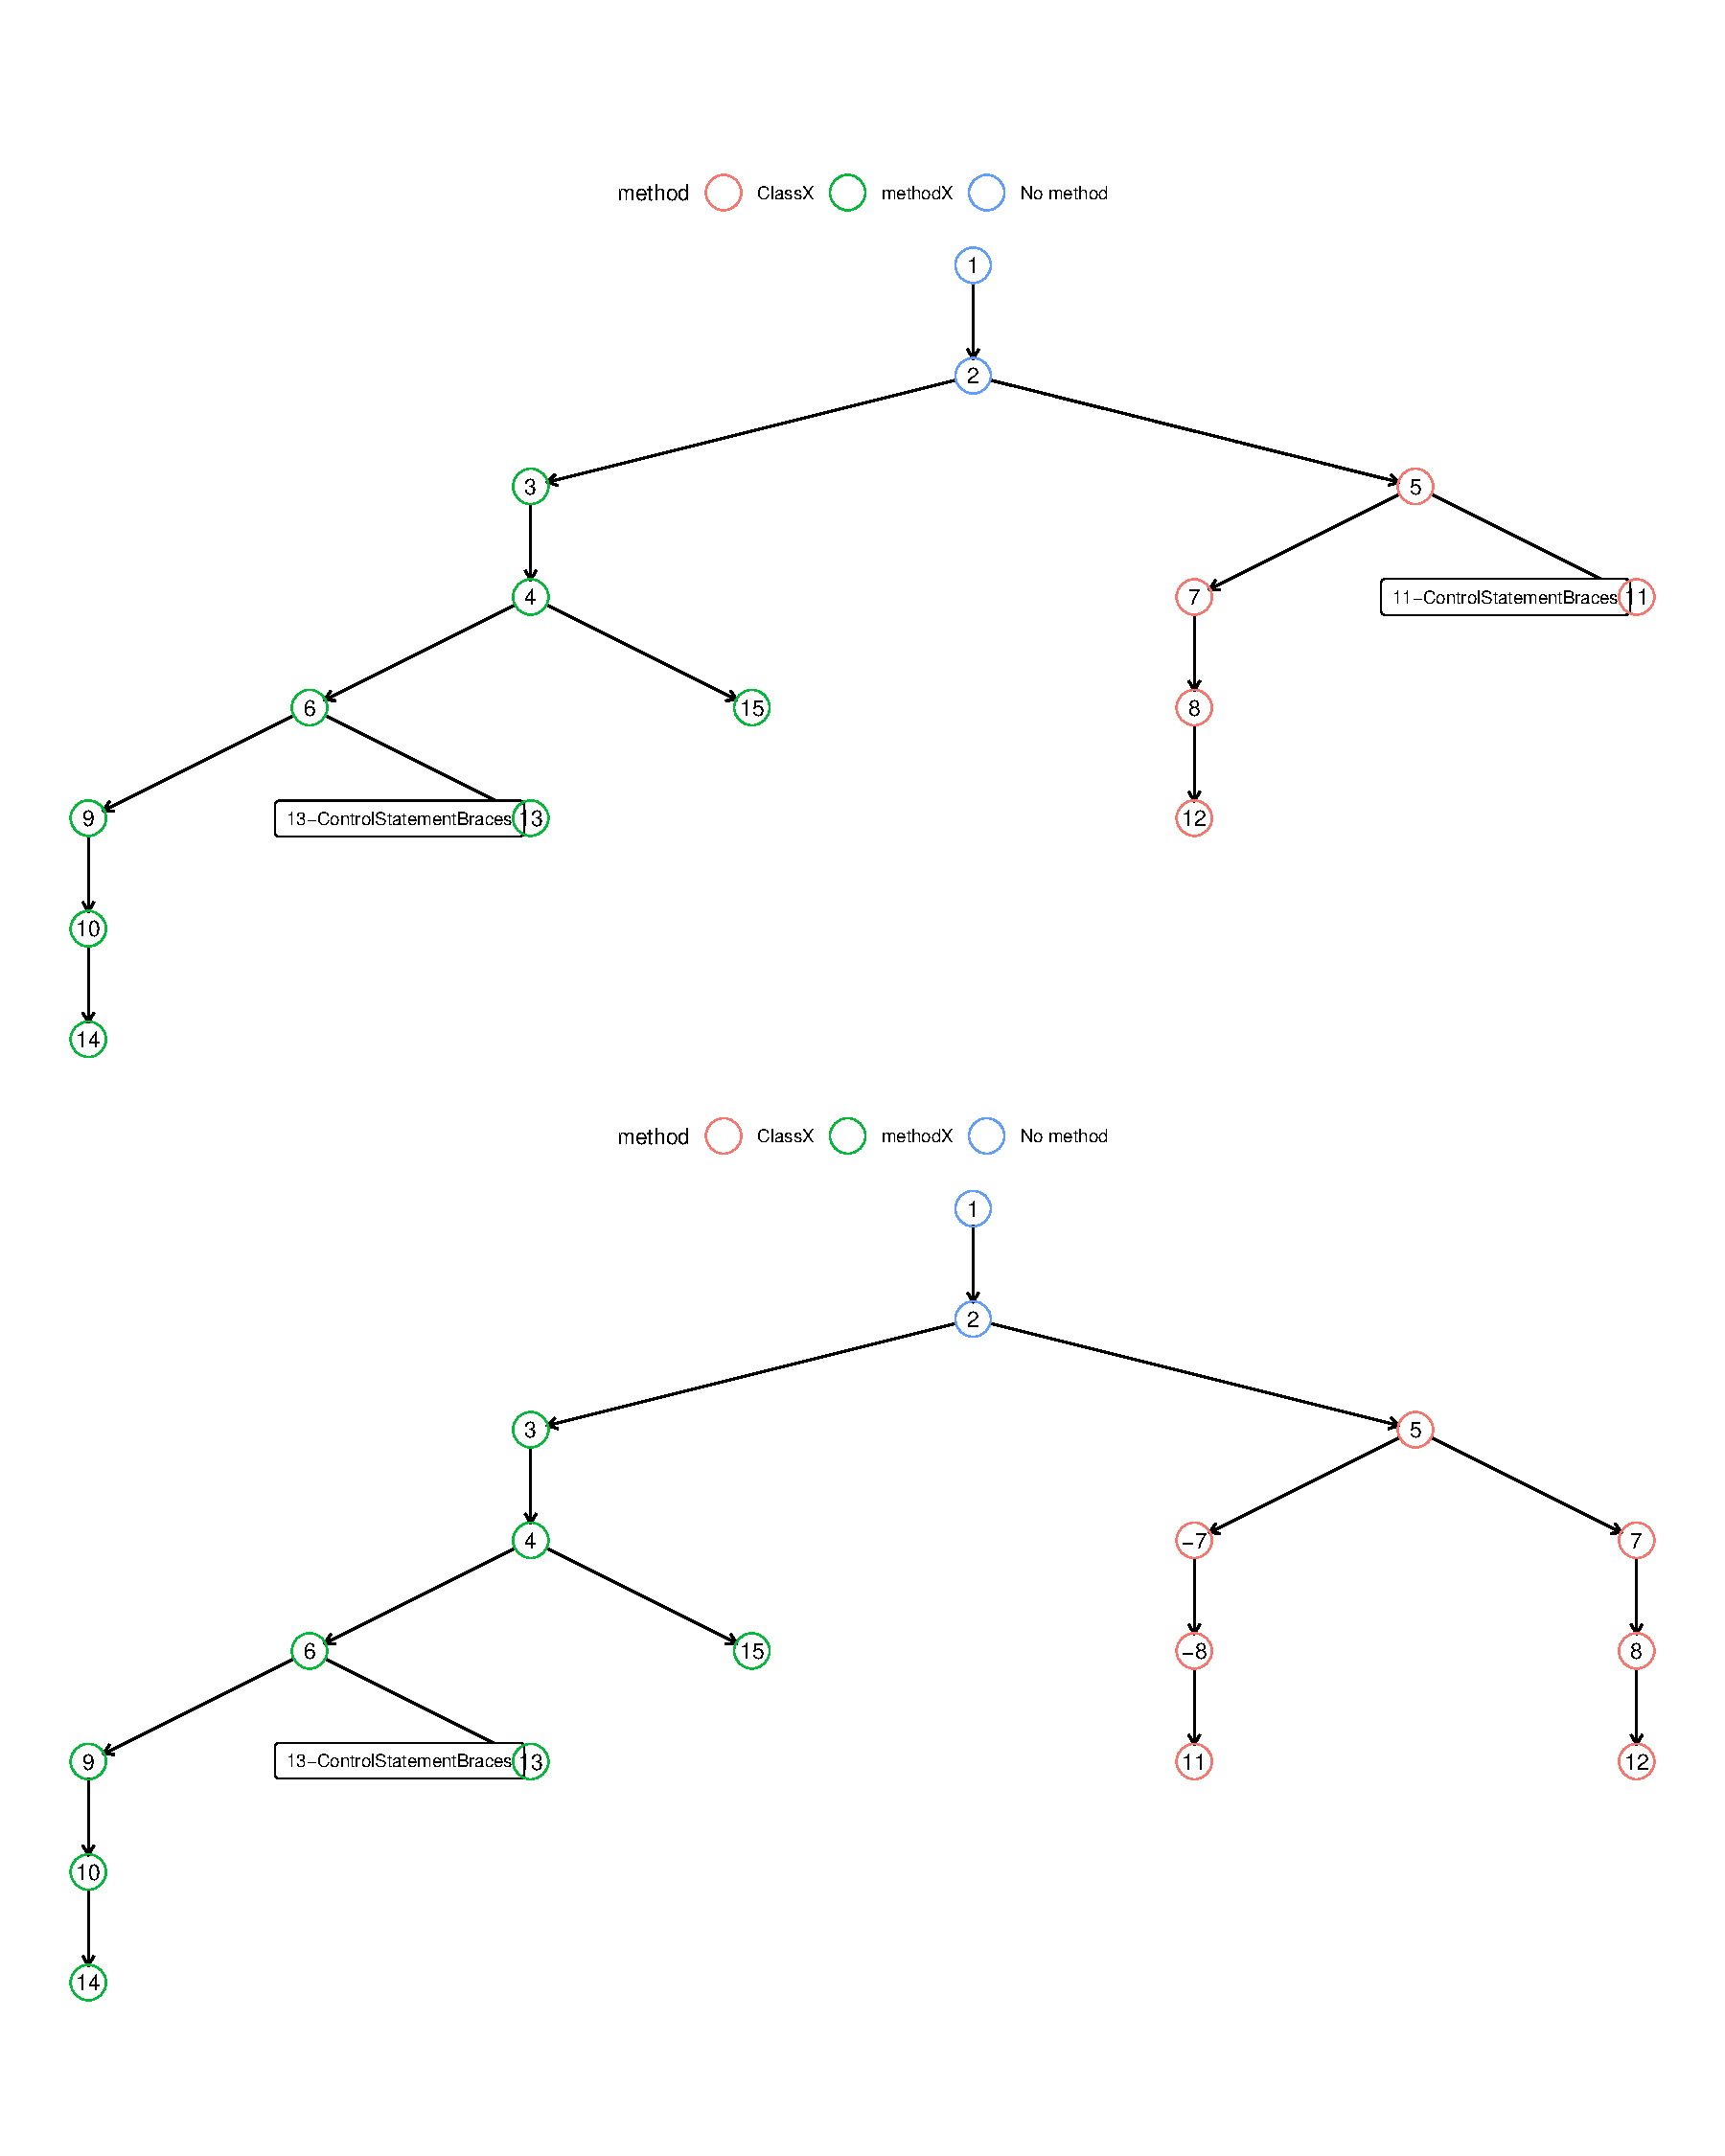
\includegraphics[width=1\linewidth]{report_files/figure-latex/unnamed-chunk-4-1} \caption{Abstract Syntax Tree \label{AST_alert_1}}\label{fig:unnamed-chunk-4}
\end{figure}

\normalsize

The algorithm generates a set of features for each pair of alerts
\((n,o)\) with one element \(n\) coming from the old version and one
element \(o\) coming from the new version. The features do not lead to a
direct conclusion. It´s necessary to create a heuristic or statistical
learning algorithm that will decide the final verdict based on the
features.

We propose the following list of features:

\begin{itemize}
\item
  Same Rule: a boolean indicator that tells if the alerts are of the
  same type
\item
  Same Group ID: a boolean indicator that tells if the alerts are
  equivalent as defined in Figure \ref{AST_groups}
\item
  Same Method Group ID: a boolean indicator that tells if the alerts
  belong to the same method. We know the alert's method following the
  path from the alert´s node to the root. The first node of the kind
  ``method'' found in this path defines the alert's method. If this is
  the same for \(o\) and for \(n\), then they belong to the same method.
\item
  Same Method Name: a boolean indicator that tells if the alerts were
  found in a method with the same name.
\item
  Same Block: a boolean indicator that shows if the \(o\) and \(n\)
  belong to the same block. It is defined the same way the ``Same
  method'' indicator is defined.
\item
  Same Code: a boolean indicator that shows the nodes that generate the
  alert have the same programming code.
\item
  Same Method Code: a boolean indicator that shows that the methods that
  contain the nodes that generate the alert have the same programming
  code.
\item
  Line distance: \(o\) and \(n\) have a begin line \(b(o)\) and \(b(n)\)
  and an end line \(e(n)\) and \(e(n)\). Line distance is
  \(abs(mean(b(o), e(o)) - mean(b(n), e(n)))\)
\item
  Normalized line distance (block size): this is the line distance but
  normalized by the size of the last common node.
\item
  Normalized line distance (method size): this is the line distance but
  normalized by the size of the last common method (if there is no
  common method, it´s normalized by the side of the compilation unit).
\item
  Normalized line distance (compilation unit size): this is the line
  distance but normalized by the size of the compilation unit.
\end{itemize}

Table \ref{table_features} shows the combinations \((n,o)\) in the
example. There are \(2 \cdot 1 = 2\) combinations whereas we have two
alerts in the old version and one alert in the new one.

\small

\begin{table}[!h]

\caption{\label{tab:unnamed-chunk-5}Resulting features\label{table_features} }
\centering
\begin{tabular}[t]{l|l|l}
\hline
Alert combination & Feature & Value\\
\hline
\rowcolor{gray!6}   & Same Rule & TRUE\\

 & Same Group ID & TRUE\\

\rowcolor{gray!6}   & Same Method Group ID & TRUE\\

 & Same Method Name & TRUE\\

\rowcolor{gray!6}   & Same Block & TRUE\\

 & Same Code & TRUE\\

\rowcolor{gray!6}   & Same Method Code & TRUE\\

 & Line Distance & 0.00\\

\rowcolor{gray!6}   & Line Distance Normalized by Block Size & 0.00\\

 & Line Distance Normalized by Method Size & 0.00\\

\multirow[t]{-11}{*}{\raggedright\arraybackslash Line (Old version):20, Line (New version):22} & Line Distance Normalized by Compilation Unit Size & 0.00\\
\hline
\end{tabular}
\end{table}

\normalsize

\small

\normalsize

\newpage

\begin{landscape}

\subsection{Example: Renaming method} \label{example_rename_method}

In this example, the new and old versions have only one alert. The
method in which the alert happens is renamed from MethodX to methodZ.

\scriptsize

\begin{Shaded}
\begin{Highlighting}[]
\CommentTok{/*  1-                 */}\KeywordTok{package}\ImportTok{ pack_x;                                                /*  1-                 */package pack_x;}                                                
\CommentTok{/*  2-                 */}                                                               \CommentTok{/*  2-                 */}                                                               
\CommentTok{/*  3-                 */}\KeywordTok{import}\ImportTok{ importX.function;                                       /*  3-                 */import importX.function;}                                       
\CommentTok{/*  4-                 */}                                                               \CommentTok{/*  4-                 */}                                                               
\CommentTok{/*  5-                 */}\KeywordTok{class}\NormalTok{ ClassX }\KeywordTok{extends}\NormalTok{ ClassY }\KeywordTok{implements}\NormalTok{ InterfX \{               }\CommentTok{/*  5-                 */}\KeywordTok{class}\NormalTok{ ClassX }\KeywordTok{extends}\NormalTok{ ClassY }\KeywordTok{implements}\NormalTok{ InterfX \{               }
\CommentTok{/*  6-                 */}    \KeywordTok{private} \DataTypeTok{long}\NormalTok{ fieldX;                                       }\CommentTok{/*  6-                 */}    \KeywordTok{private} \DataTypeTok{long}\NormalTok{ fieldX;                                       }
\CommentTok{/*  7-                 */}                                                               \CommentTok{/*  7-                 */}                                                               
\CommentTok{/*  8-                 */}    \FunctionTok{ClassX}\NormalTok{(}\DataTypeTok{int}\NormalTok{ paramX, }\DataTypeTok{double}\NormalTok{ paramY) \{                                }\CommentTok{/*  8-                 */}    \FunctionTok{ClassX}\NormalTok{(}\DataTypeTok{int}\NormalTok{ paramX, }\DataTypeTok{double}\NormalTok{ paramY) \{                                }
\CommentTok{/*  9-                 */}        \DataTypeTok{int}\NormalTok{ varX = }\FunctionTok{function}\NormalTok{(paramX, paramY);                          }\CommentTok{/*  9-                 */}        \DataTypeTok{int}\NormalTok{ varX = }\FunctionTok{function}\NormalTok{(paramX, paramY);                           }
\CommentTok{/*   -                 *//*XXXXXXXXXXXXXXXXXXXXXXXXXXXXXXXXXXXXXX*/}                     \CommentTok{/* 10-                 */}        \KeywordTok{if}\NormalTok{ (varX == }\DecValTok{0}\NormalTok{)                                         }
\CommentTok{/* 10-                 */}        \KeywordTok{if}\NormalTok{ (varX == }\DecValTok{0}\NormalTok{)\{                                        }\CommentTok{/*   -                 *//*XXXXXXXXXXXXXXXXXXXXXXXXXXXXXXXXXXXXXX*/}                     
\CommentTok{/*   -                 *//*XXXXXXXXXXXXXXXXXXXXXXXXXXXXXXXXXXXXXX*/}                     \CommentTok{/* 11-                 */}\NormalTok{        \{                                                      }
\CommentTok{/* 11-                 */}            \KeywordTok{this}\NormalTok{.}\FunctionTok{fieldX}\NormalTok{ = }\DecValTok{1}\NormalTok{;                                   }\CommentTok{/* 12-                 */}            \KeywordTok{this}\NormalTok{.}\FunctionTok{fieldX}\NormalTok{ = }\DecValTok{1}\NormalTok{;                                   }
\CommentTok{/* 12-                 */}\NormalTok{        \}                                                      }\CommentTok{/*   -                 *//*XXXXXXXXXXXXXXXXXXXXXXXXXXXXXXXXXXXXXX*/}                     
\CommentTok{/*   -                 *//*XXXXXXXXXXXXXXXXXXXXXXXXXXXXXXXXXXXXXX*/}                     \CommentTok{/* 13-                 */}\NormalTok{        \}                                                                }
\CommentTok{/* 13-                 */}        \KeywordTok{else}\NormalTok{\{                                                  }\CommentTok{/* 14-                 */}        \KeywordTok{else}\NormalTok{\{                                                  }
\CommentTok{/* 14-                 */}            \KeywordTok{this}\NormalTok{.}\FunctionTok{fieldX}\NormalTok{ = }\DecValTok{0}\NormalTok{;                                   }\CommentTok{/* 15-                 */}            \KeywordTok{this}\NormalTok{.}\FunctionTok{fieldX}\NormalTok{ = }\DecValTok{0}\NormalTok{;                                   }
\CommentTok{/* 15-                 */}\NormalTok{        \}                                                      }\CommentTok{/* 16-                 */}\NormalTok{        \}                                                      }
\CommentTok{/* 16-                 */}\NormalTok{    \}                                                          }\CommentTok{/* 17-                 */}\NormalTok{    \}                                                          }
\CommentTok{/* 17-                 */}    \AttributeTok{@Override}                                                  \CommentTok{/* 18-                 */}    \AttributeTok{@Override}                                                  
\CommentTok{/* 18-                 */}    \KeywordTok{public} \DataTypeTok{int} \FunctionTok{methodX}\NormalTok{(}\DataTypeTok{int}\NormalTok{ paramW, }\BuiltInTok{Boolean}\NormalTok{ paramZ)             }\CommentTok{/*   -                 *//*XXXXXXXXXXXXXXXXXXXXXXXXXXXXXXXXXXXXXX*/}                     
\CommentTok{/*   -                 *//*XXXXXXXXXXXXXXXXXXXXXXXXXXXXXXXXXXXXXX*/}                     \CommentTok{/* 19-                 */}    \KeywordTok{public} \DataTypeTok{int} \FunctionTok{methodZ}\NormalTok{(}\DataTypeTok{int}\NormalTok{ paramW, }\BuiltInTok{Boolean}\NormalTok{ paramZ)             }
\CommentTok{/* 19-                 */}\NormalTok{    \{                                                          }\CommentTok{/* 20-                 */}\NormalTok{    \{                                                          }
\CommentTok{/* 20-                 */}        \KeywordTok{if}\NormalTok{ (paramZ)                                            }\CommentTok{/* 21-                 */}        \KeywordTok{if}\NormalTok{ (paramZ)                                            }
\CommentTok{/* 21-ControlStateme   */}\NormalTok{            fieldX = paramW;                                   }\CommentTok{/* 22-ControlStateme   */}\NormalTok{            fieldX = paramW;                                   }
\CommentTok{/* 22-                 */}        \KeywordTok{else}\NormalTok{\{                                                  }\CommentTok{/* 23-                 */}        \KeywordTok{else}\NormalTok{\{                                                  }
\CommentTok{/* 23-                 */}\NormalTok{            fieldX = }\DecValTok{0}\NormalTok{;                                        }\CommentTok{/* 24-                 */}\NormalTok{            fieldX = }\DecValTok{0}\NormalTok{;                                        }
\CommentTok{/* 24-                 */}\NormalTok{        \}                                                      }\CommentTok{/* 25-                 */}\NormalTok{        \}                                                      }
\CommentTok{/* 25-                 */}        \KeywordTok{return}\NormalTok{ paramW + }\KeywordTok{this}\NormalTok{.}\FunctionTok{fieldX}\NormalTok{;                           }\CommentTok{/* 26-                 */}        \KeywordTok{return}\NormalTok{ paramW + }\KeywordTok{this}\NormalTok{.}\FunctionTok{fieldX}\NormalTok{;                           }
\CommentTok{/* 26-                 */}\NormalTok{     \}                                                         }\CommentTok{/* 27-                 */}\NormalTok{     \}                                                         }
\CommentTok{/* 27-                 */}\NormalTok{\}                                                              }\CommentTok{/* 28-                 */}\NormalTok{\}                                                              }
\end{Highlighting}
\end{Shaded}

\normalsize

\begin{figure}
\centering

\includegraphics{figures/fake.png}
\caption{Comparison between old and new version
\label{comparison_rename}}
\end{figure}

\end{landscape}

\newpage

In the Table \ref{features_rename} we can see that the features ``Same
Method Name'' and ``Same Method Group ID'' are now FALSE.

\small

\begin{table}[!h]

\caption{\label{tab:unnamed-chunk-7}Resulting features: rename method example \label{features_rename} }
\centering
\begin{tabular}[t]{l|l|l}
\hline
Alert combination & Feature & Value\\
\hline
\rowcolor{gray!6}   & Same Rule & TRUE\\

 & Same Group ID & TRUE\\

\rowcolor{gray!6}   & Same Method Group ID & FALSE\\

 & Same Method Name & FALSE\\

\rowcolor{gray!6}   & Same Block & TRUE\\

 & Same Code & TRUE\\

\rowcolor{gray!6}   & Same Method Code & FALSE\\

 & Line Distance & 0.00\\

\rowcolor{gray!6}   & Line Distance Normalized by Block Size & 0.00\\

 & Line Distance Normalized by Method Size & 0.00\\

\multirow[t]{-11}{*}{\raggedright\arraybackslash Line (Old version):21, Line (New version):22} & Line Distance Normalized by Compilation Unit Size & 0.00\\
\hline
\end{tabular}
\end{table}

\normalsize

\newpage

\begin{landscape}

\subsection{Example: including a statement before} \label{example_including_statement}

\small

\normalsize

In this example, a new statement is included before the alert.

\small

\normalsize

\scriptsize

\begin{Shaded}
\begin{Highlighting}[]
\CommentTok{/*  1-                 */}\KeywordTok{package}\ImportTok{ pack_x;                                                /*  1-                 */package pack_x;}                                                
\CommentTok{/*  2-                 */}                                                               \CommentTok{/*  2-                 */}                                                               
\CommentTok{/*  3-                 */}\KeywordTok{import}\ImportTok{ importX.function;                                       /*  3-                 */import importX.function;}                                       
\CommentTok{/*  4-                 */}                                                               \CommentTok{/*  4-                 */}                                                               
\CommentTok{/*  5-                 */}\KeywordTok{class}\NormalTok{ ClassX }\KeywordTok{extends}\NormalTok{ ClassY }\KeywordTok{implements}\NormalTok{ InterfX \{               }\CommentTok{/*  5-                 */}\KeywordTok{class}\NormalTok{ ClassX }\KeywordTok{extends}\NormalTok{ ClassY }\KeywordTok{implements}\NormalTok{ InterfX \{               }
\CommentTok{/*  6-                 */}    \KeywordTok{private} \DataTypeTok{long}\NormalTok{ fieldX;                                       }\CommentTok{/*  6-                 */}    \KeywordTok{private} \DataTypeTok{long}\NormalTok{ fieldX;                                       }
\CommentTok{/*  7-                 */}                                                               \CommentTok{/*  7-                 */}                                                               
\CommentTok{/*  8-                 */}    \FunctionTok{ClassX}\NormalTok{(}\DataTypeTok{int}\NormalTok{ paramX, }\DataTypeTok{double}\NormalTok{ paramY) \{                                }\CommentTok{/*  8-                 */}    \FunctionTok{ClassX}\NormalTok{(}\DataTypeTok{int}\NormalTok{ paramX, }\DataTypeTok{double}\NormalTok{ paramY) \{                                }
\CommentTok{/*  9-                 */}        \DataTypeTok{int}\NormalTok{ varX = }\FunctionTok{function}\NormalTok{(paramX, paramY);                          }\CommentTok{/*  9-                 */}        \DataTypeTok{int}\NormalTok{ varX = }\FunctionTok{function}\NormalTok{(paramX, paramY);                           }
\CommentTok{/*   -                 *//*XXXXXXXXXXXXXXXXXXXXXXXXXXXXXXXXXXXXXX*/}                     \CommentTok{/* 10-                 */}        \KeywordTok{if}\NormalTok{ (varX == }\DecValTok{0}\NormalTok{)                                         }
\CommentTok{/* 10-                 */}        \KeywordTok{if}\NormalTok{ (varX == }\DecValTok{0}\NormalTok{)\{                                        }\CommentTok{/*   -                 *//*XXXXXXXXXXXXXXXXXXXXXXXXXXXXXXXXXXXXXX*/}                     
\CommentTok{/*   -                 *//*XXXXXXXXXXXXXXXXXXXXXXXXXXXXXXXXXXXXXX*/}                     \CommentTok{/* 11-                 */}\NormalTok{        \{                                                      }
\CommentTok{/* 11-                 */}            \KeywordTok{this}\NormalTok{.}\FunctionTok{fieldX}\NormalTok{ = }\DecValTok{1}\NormalTok{;                                   }\CommentTok{/* 12-                 */}            \KeywordTok{this}\NormalTok{.}\FunctionTok{fieldX}\NormalTok{ = }\DecValTok{1}\NormalTok{;                                   }
\CommentTok{/* 12-                 */}\NormalTok{        \}                                                      }\CommentTok{/*   -                 *//*XXXXXXXXXXXXXXXXXXXXXXXXXXXXXXXXXXXXXX*/}                     
\CommentTok{/*   -                 *//*XXXXXXXXXXXXXXXXXXXXXXXXXXXXXXXXXXXXXX*/}                     \CommentTok{/* 13-                 */}\NormalTok{        \}                                                                }
\CommentTok{/* 13-                 */}        \KeywordTok{else}\NormalTok{\{                                                  }\CommentTok{/* 14-                 */}        \KeywordTok{else}\NormalTok{\{                                                  }
\CommentTok{/* 14-                 */}            \KeywordTok{this}\NormalTok{.}\FunctionTok{fieldX}\NormalTok{ = }\DecValTok{0}\NormalTok{;                                   }\CommentTok{/* 15-                 */}            \KeywordTok{this}\NormalTok{.}\FunctionTok{fieldX}\NormalTok{ = }\DecValTok{0}\NormalTok{;                                   }
\CommentTok{/* 15-                 */}\NormalTok{        \}                                                      }\CommentTok{/* 16-                 */}\NormalTok{        \}                                                      }
\CommentTok{/* 16-                 */}\NormalTok{    \}                                                          }\CommentTok{/* 17-                 */}\NormalTok{    \}                                                          }
\CommentTok{/* 17-                 */}    \AttributeTok{@Override}                                                  \CommentTok{/* 18-                 */}    \AttributeTok{@Override}                                                  
\CommentTok{/* 18-                 */}    \KeywordTok{public} \DataTypeTok{int} \FunctionTok{methodX}\NormalTok{(}\DataTypeTok{int}\NormalTok{ paramW, }\BuiltInTok{Boolean}\NormalTok{ paramZ)             }\CommentTok{/* 19-                 */}    \KeywordTok{public} \DataTypeTok{int} \FunctionTok{methodX}\NormalTok{(}\DataTypeTok{int}\NormalTok{ paramW, }\BuiltInTok{Boolean}\NormalTok{ paramZ)             }
\CommentTok{/* 19-                 */}\NormalTok{    \{                                                          }\CommentTok{/* 20-                 */}\NormalTok{    \{                                                          }
\CommentTok{/*   -                 *//*XXXXXXXXXXXXXXXXXXXXXXXXXXXXXXXXXXXXXX*/}                     \CommentTok{/* 21-                 */}\NormalTok{        paramT = }\DecValTok{0}\NormalTok{;                                            }
\CommentTok{/* 20-                 */}        \KeywordTok{if}\NormalTok{ (paramZ)                                            }\CommentTok{/* 22-                 */}        \KeywordTok{if}\NormalTok{ (paramZ)                                            }
\CommentTok{/* 21-ControlStateme   */}\NormalTok{            fieldX = paramW;                                   }\CommentTok{/* 23-ControlStateme   */}\NormalTok{            fieldX = paramW;                                   }
\CommentTok{/* 22-                 */}        \KeywordTok{else}\NormalTok{\{                                                  }\CommentTok{/* 24-                 */}        \KeywordTok{else}\NormalTok{\{                                                  }
\CommentTok{/* 23-                 */}\NormalTok{            fieldX = }\DecValTok{0}\NormalTok{;                                        }\CommentTok{/* 25-                 */}\NormalTok{            fieldX = }\DecValTok{0}\NormalTok{;                                        }
\CommentTok{/* 24-                 */}\NormalTok{        \}                                                      }\CommentTok{/* 26-                 */}\NormalTok{        \}                                                      }
\CommentTok{/* 25-                 */}        \KeywordTok{return}\NormalTok{ paramW + }\KeywordTok{this}\NormalTok{.}\FunctionTok{fieldX}\NormalTok{;                           }\CommentTok{/* 27-                 */}        \KeywordTok{return}\NormalTok{ paramW + }\KeywordTok{this}\NormalTok{.}\FunctionTok{fieldX}\NormalTok{;                           }
\CommentTok{/* 26-                 */}\NormalTok{     \}                                                         }\CommentTok{/* 28-                 */}\NormalTok{     \}                                                         }
\CommentTok{/* 27-                 */}\NormalTok{\}                                                              }\CommentTok{/* 29-                 */}\NormalTok{\}                                                              }
\end{Highlighting}
\end{Shaded}

\normalsize

\begin{figure}
\centering

\includegraphics{figures/fake.png}
\caption{Comparison between old and new version
\label{comparison_include_statement_before}}
\end{figure}

\end{landscape}

\newpage

In the Table \ref{include_statement_before} we can see that the features
are not affected by this new statement.

\small

\begin{table}[!h]

\caption{\label{tab:unnamed-chunk-10}Resulting features: statement included before \label{include_statement_before} }
\centering
\begin{tabular}[t]{l|l|l}
\hline
Alert combination & Feature & Value\\
\hline
\rowcolor{gray!6}   & Same Rule & TRUE\\

 & Same Group ID & TRUE\\

\rowcolor{gray!6}   & Same Method Group ID & TRUE\\

 & Same Method Name & TRUE\\

\rowcolor{gray!6}   & Same Block & TRUE\\

 & Same Code & TRUE\\

\rowcolor{gray!6}   & Same Method Code & FALSE\\

 & Line Distance & 0.00\\

\rowcolor{gray!6}   & Line Distance Normalized by Block Size & 0.00\\

 & Line Distance Normalized by Method Size & 0.00\\

\multirow[t]{-11}{*}{\raggedright\arraybackslash Line (Old version):21, Line (New version):23} & Line Distance Normalized by Compilation Unit Size & 0.00\\
\hline
\end{tabular}
\end{table}

\normalsize

\newpage

\begin{landscape}

\subsection{Example: nesting the alert in an if statement} \label{example_nested_in_other_if}

\small

\normalsize

\scriptsize

\begin{Shaded}
\begin{Highlighting}[]
\CommentTok{/*  1-                 */}\KeywordTok{package}\ImportTok{ pack_x;                                                /*  1-                 */package pack_x;}                                                
\CommentTok{/*  2-                 */}                                                               \CommentTok{/*  2-                 */}                                                               
\CommentTok{/*  3-                 */}\KeywordTok{import}\ImportTok{ importX.function;                                       /*  3-                 */import importX.function;}                                       
\CommentTok{/*  4-                 */}                                                               \CommentTok{/*  4-                 */}                                                               
\CommentTok{/*  5-                 */}\KeywordTok{class}\NormalTok{ ClassX }\KeywordTok{extends}\NormalTok{ ClassY }\KeywordTok{implements}\NormalTok{ InterfX \{               }\CommentTok{/*  5-                 */}\KeywordTok{class}\NormalTok{ ClassX }\KeywordTok{extends}\NormalTok{ ClassY }\KeywordTok{implements}\NormalTok{ InterfX \{               }
\CommentTok{/*  6-                 */}    \KeywordTok{private} \DataTypeTok{long}\NormalTok{ fieldX;                                       }\CommentTok{/*  6-                 */}    \KeywordTok{private} \DataTypeTok{long}\NormalTok{ fieldX;                                       }
\CommentTok{/*  7-                 */}                                                               \CommentTok{/*  7-                 */}                                                               
\CommentTok{/*  8-                 */}    \FunctionTok{ClassX}\NormalTok{(}\DataTypeTok{int}\NormalTok{ paramX, }\DataTypeTok{double}\NormalTok{ paramY) \{                                }\CommentTok{/*  8-                 */}    \FunctionTok{ClassX}\NormalTok{(}\DataTypeTok{int}\NormalTok{ paramX, }\DataTypeTok{double}\NormalTok{ paramY) \{                                }
\CommentTok{/*  9-                 */}        \DataTypeTok{int}\NormalTok{ varX = }\FunctionTok{function}\NormalTok{(paramX, paramY);                          }\CommentTok{/*  9-                 */}        \DataTypeTok{int}\NormalTok{ varX = }\FunctionTok{function}\NormalTok{(paramX, paramY);                           }
\CommentTok{/*   -                 *//*XXXXXXXXXXXXXXXXXXXXXXXXXXXXXXXXXXXXXX*/}                     \CommentTok{/* 10-                 */}        \KeywordTok{if}\NormalTok{ (varX == }\DecValTok{0}\NormalTok{)                                         }
\CommentTok{/* 10-                 */}        \KeywordTok{if}\NormalTok{ (varX == }\DecValTok{0}\NormalTok{)\{                                        }\CommentTok{/*   -                 *//*XXXXXXXXXXXXXXXXXXXXXXXXXXXXXXXXXXXXXX*/}                     
\CommentTok{/*   -                 *//*XXXXXXXXXXXXXXXXXXXXXXXXXXXXXXXXXXXXXX*/}                     \CommentTok{/* 11-                 */}\NormalTok{        \{                                                      }
\CommentTok{/* 11-                 */}            \KeywordTok{this}\NormalTok{.}\FunctionTok{fieldX}\NormalTok{ = }\DecValTok{1}\NormalTok{;                                   }\CommentTok{/* 12-                 */}            \KeywordTok{this}\NormalTok{.}\FunctionTok{fieldX}\NormalTok{ = }\DecValTok{1}\NormalTok{;                                   }
\CommentTok{/* 12-                 */}\NormalTok{        \}                                                      }\CommentTok{/*   -                 *//*XXXXXXXXXXXXXXXXXXXXXXXXXXXXXXXXXXXXXX*/}                     
\CommentTok{/*   -                 *//*XXXXXXXXXXXXXXXXXXXXXXXXXXXXXXXXXXXXXX*/}                     \CommentTok{/* 13-                 */}\NormalTok{        \}                                                                }
\CommentTok{/* 13-                 */}        \KeywordTok{else}\NormalTok{\{                                                  }\CommentTok{/* 14-                 */}        \KeywordTok{else}\NormalTok{\{                                                  }
\CommentTok{/* 14-                 */}            \KeywordTok{this}\NormalTok{.}\FunctionTok{fieldX}\NormalTok{ = }\DecValTok{0}\NormalTok{;                                   }\CommentTok{/* 15-                 */}            \KeywordTok{this}\NormalTok{.}\FunctionTok{fieldX}\NormalTok{ = }\DecValTok{0}\NormalTok{;                                   }
\CommentTok{/* 15-                 */}\NormalTok{        \}                                                      }\CommentTok{/* 16-                 */}\NormalTok{        \}                                                      }
\CommentTok{/* 16-                 */}\NormalTok{    \}                                                          }\CommentTok{/* 17-                 */}\NormalTok{    \}                                                          }
\CommentTok{/* 17-                 */}    \AttributeTok{@Override}                                                  \CommentTok{/* 18-                 */}    \AttributeTok{@Override}                                                  
\CommentTok{/* 18-                 */}    \KeywordTok{public} \DataTypeTok{int} \FunctionTok{methodX}\NormalTok{(}\DataTypeTok{int}\NormalTok{ paramW, }\BuiltInTok{Boolean}\NormalTok{ paramZ)             }\CommentTok{/* 19-                 */}    \KeywordTok{public} \DataTypeTok{int} \FunctionTok{methodX}\NormalTok{(}\DataTypeTok{int}\NormalTok{ paramW, }\BuiltInTok{Boolean}\NormalTok{ paramZ)             }
\CommentTok{/* 19-                 */}\NormalTok{    \{                                                          }\CommentTok{/* 20-                 */}\NormalTok{    \{                                                          }
\CommentTok{/* 20-                 */}        \KeywordTok{if}\NormalTok{ (paramZ)                                            }\CommentTok{/*   -                 *//*XXXXXXXXXXXXXXXXXXXXXXXXXXXXXXXXXXXXXX*/}                     
\CommentTok{/*   -                 *//*XXXXXXXXXXXXXXXXXXXXXXXXXXXXXXXXXXXXXX*/}                     \CommentTok{/* 21-                 */}        \KeywordTok{if}\NormalTok{(paramZ == }\DecValTok{0}\NormalTok{)\{                                       }
\CommentTok{/* 21-ControlStateme   */}\NormalTok{            fieldX = paramW;                                   }\CommentTok{/*   -                 *//*XXXXXXXXXXXXXXXXXXXXXXXXXXXXXXXXXXXXXX*/}                     
\CommentTok{/*   -                 *//*XXXXXXXXXXXXXXXXXXXXXXXXXXXXXXXXXXXXXX*/}                     \CommentTok{/* 22-                 */}            \KeywordTok{if}\NormalTok{ (paramZ)                                        }
\CommentTok{/*   -                 *//*XXXXXXXXXXXXXXXXXXXXXXXXXXXXXXXXXXXXXX*/}                     \CommentTok{/* 23-ControlStateme   */}\NormalTok{                fieldX = paramW;                               }
\CommentTok{/* 23-                 */}\NormalTok{            fieldX = }\DecValTok{0}\NormalTok{;                                        }\CommentTok{/*   -                 *//*XXXXXXXXXXXXXXXXXXXXXXXXXXXXXXXXXXXXXX*/}                     
\CommentTok{/*   -                 *//*XXXXXXXXXXXXXXXXXXXXXXXXXXXXXXXXXXXXXX*/}                     \CommentTok{/* 24-                 */}            \KeywordTok{else}\NormalTok{\{                                              }
\CommentTok{/*   -                 *//*XXXXXXXXXXXXXXXXXXXXXXXXXXXXXXXXXXXXXX*/}                     \CommentTok{/* 25-                 */}\NormalTok{                fieldX = }\DecValTok{0}\NormalTok{;                                    }
\CommentTok{/*   -                 *//*XXXXXXXXXXXXXXXXXXXXXXXXXXXXXXXXXXXXXX*/}                     \CommentTok{/* 26-                 */}\NormalTok{            \}                                                  }
\CommentTok{/*   -                 *//*XXXXXXXXXXXXXXXXXXXXXXXXXXXXXXXXXXXXXX*/}                     \CommentTok{/* 27-                 */}\NormalTok{        \}                                                      }
\CommentTok{/* 22-                 */}        \KeywordTok{else}\NormalTok{\{                                                  }\CommentTok{/* 28-                 */}        \KeywordTok{else}\NormalTok{\{                                                  }
\CommentTok{/*   -                 *//*XXXXXXXXXXXXXXXXXXXXXXXXXXXXXXXXXXXXXX*/}                     \CommentTok{/* 29-                 */}\NormalTok{            fieldX = }\DecValTok{1}\NormalTok{;                                        }
\CommentTok{/* 24-                 */}\NormalTok{        \}                                                      }\CommentTok{/* 30-                 */}\NormalTok{        \}                                                      }
\CommentTok{/* 25-                 */}        \KeywordTok{return}\NormalTok{ paramW + }\KeywordTok{this}\NormalTok{.}\FunctionTok{fieldX}\NormalTok{;                           }\CommentTok{/* 31-                 */}        \KeywordTok{return}\NormalTok{ paramW + }\KeywordTok{this}\NormalTok{.}\FunctionTok{fieldX}\NormalTok{;                           }
\CommentTok{/* 26-                 */}\NormalTok{     \}                                                         }\CommentTok{/* 32-                 */}\NormalTok{     \}                                                         }
\CommentTok{/* 27-                 */}\NormalTok{\}                                                              }\CommentTok{/* 33-                 */}\NormalTok{\}                                                              }
\end{Highlighting}
\end{Shaded}

\normalsize

\begin{figure}
\centering

\includegraphics{figures/fake.png}
\caption{Comparison between old and new version
\label{comparison_nested_in_other_if}}
\end{figure}

\end{landscape}

\newpage

In the Table \ref{nested_in_other_if} we can see that the algorithm does
not recognize the two nodes as equivalent, but other features can lead
us to the conclusion that the alert is still open.

\small

\begin{table}[!h]

\caption{\label{tab:unnamed-chunk-12}Resulting features: statement included before \label{nested_in_other_if} }
\centering
\begin{tabular}[t]{l|l|l}
\hline
Alert combination & Feature & Value\\
\hline
\rowcolor{gray!6}   & Same Rule & TRUE\\

 & Same Group ID & FALSE\\

\rowcolor{gray!6}   & Same Method Group ID & TRUE\\

 & Same Method Name & TRUE\\

\rowcolor{gray!6}   & Same Block & FALSE\\

 & Same Code & TRUE\\

\rowcolor{gray!6}   & Same Method Code & FALSE\\

 & Line Distance & 2.00\\

\rowcolor{gray!6}   & Line Distance Normalized by Block Size & 0.13\\

 & Line Distance Normalized by Method Size & 0.12\\

\multirow[t]{-11}{*}{\raggedright\arraybackslash Line (Old version):21, Line (New version):23} & Line Distance Normalized by Compilation Unit Size & 0.05\\
\hline
\end{tabular}
\end{table}

\normalsize

\newpage

\begin{landscape}

\subsection{Example: editing the line that generates the alert} \label{example_editing_line}

\small

\normalsize

\scriptsize

\begin{Shaded}
\begin{Highlighting}[]
\CommentTok{/*  1-                 */}\KeywordTok{package}\ImportTok{ pack_x;                                                /*  1-                 */package pack_x;}                                                
\CommentTok{/*  2-                 */}                                                               \CommentTok{/*  2-                 */}                                                               
\CommentTok{/*  3-                 */}\KeywordTok{import}\ImportTok{ importX.function;                                       /*  3-                 */import importX.function;}                                       
\CommentTok{/*  4-                 */}                                                               \CommentTok{/*  4-                 */}                                                               
\CommentTok{/*  5-                 */}\KeywordTok{class}\NormalTok{ ClassX }\KeywordTok{extends}\NormalTok{ ClassY }\KeywordTok{implements}\NormalTok{ InterfX \{               }\CommentTok{/*  5-                 */}\KeywordTok{class}\NormalTok{ ClassX }\KeywordTok{extends}\NormalTok{ ClassY }\KeywordTok{implements}\NormalTok{ InterfX \{               }
\CommentTok{/*  6-                 */}    \KeywordTok{private} \DataTypeTok{long}\NormalTok{ fieldX;                                       }\CommentTok{/*  6-                 */}    \KeywordTok{private} \DataTypeTok{long}\NormalTok{ fieldX;                                       }
\CommentTok{/*  7-                 */}                                                               \CommentTok{/*  7-                 */}                                                               
\CommentTok{/*  8-                 */}    \FunctionTok{ClassX}\NormalTok{(}\DataTypeTok{int}\NormalTok{ paramX, }\DataTypeTok{double}\NormalTok{ paramY) \{                                }\CommentTok{/*  8-                 */}    \FunctionTok{ClassX}\NormalTok{(}\DataTypeTok{int}\NormalTok{ paramX, }\DataTypeTok{double}\NormalTok{ paramY) \{                                }
\CommentTok{/*  9-                 */}        \DataTypeTok{int}\NormalTok{ varX = }\FunctionTok{function}\NormalTok{(paramX, paramY);                          }\CommentTok{/*  9-                 */}        \DataTypeTok{int}\NormalTok{ varX = }\FunctionTok{function}\NormalTok{(paramX, paramY);                           }
\CommentTok{/*   -                 *//*XXXXXXXXXXXXXXXXXXXXXXXXXXXXXXXXXXXXXX*/}                     \CommentTok{/* 10-                 */}        \KeywordTok{if}\NormalTok{ (varX == }\DecValTok{0}\NormalTok{)                                         }
\CommentTok{/* 10-                 */}        \KeywordTok{if}\NormalTok{ (varX == }\DecValTok{0}\NormalTok{)\{                                        }\CommentTok{/*   -                 *//*XXXXXXXXXXXXXXXXXXXXXXXXXXXXXXXXXXXXXX*/}                     
\CommentTok{/*   -                 *//*XXXXXXXXXXXXXXXXXXXXXXXXXXXXXXXXXXXXXX*/}                     \CommentTok{/* 11-                 */}\NormalTok{        \{                                                      }
\CommentTok{/* 11-                 */}            \KeywordTok{this}\NormalTok{.}\FunctionTok{fieldX}\NormalTok{ = }\DecValTok{1}\NormalTok{;                                   }\CommentTok{/* 12-                 */}            \KeywordTok{this}\NormalTok{.}\FunctionTok{fieldX}\NormalTok{ = }\DecValTok{1}\NormalTok{;                                   }
\CommentTok{/* 12-                 */}\NormalTok{        \}                                                      }\CommentTok{/*   -                 *//*XXXXXXXXXXXXXXXXXXXXXXXXXXXXXXXXXXXXXX*/}                     
\CommentTok{/*   -                 *//*XXXXXXXXXXXXXXXXXXXXXXXXXXXXXXXXXXXXXX*/}                     \CommentTok{/* 13-                 */}\NormalTok{        \}                                                                }
\CommentTok{/* 13-                 */}        \KeywordTok{else}\NormalTok{\{                                                  }\CommentTok{/* 14-                 */}        \KeywordTok{else}\NormalTok{\{                                                  }
\CommentTok{/* 14-                 */}            \KeywordTok{this}\NormalTok{.}\FunctionTok{fieldX}\NormalTok{ = }\DecValTok{0}\NormalTok{;                                   }\CommentTok{/* 15-                 */}            \KeywordTok{this}\NormalTok{.}\FunctionTok{fieldX}\NormalTok{ = }\DecValTok{0}\NormalTok{;                                   }
\CommentTok{/* 15-                 */}\NormalTok{        \}                                                      }\CommentTok{/* 16-                 */}\NormalTok{        \}                                                      }
\CommentTok{/* 16-                 */}\NormalTok{    \}                                                          }\CommentTok{/* 17-                 */}\NormalTok{    \}                                                          }
\CommentTok{/* 17-                 */}    \AttributeTok{@Override}                                                  \CommentTok{/* 18-                 */}    \AttributeTok{@Override}                                                  
\CommentTok{/* 18-                 */}    \KeywordTok{public} \DataTypeTok{int} \FunctionTok{methodX}\NormalTok{(}\DataTypeTok{int}\NormalTok{ paramW, }\BuiltInTok{Boolean}\NormalTok{ paramZ)             }\CommentTok{/* 19-                 */}    \KeywordTok{public} \DataTypeTok{int} \FunctionTok{methodX}\NormalTok{(}\DataTypeTok{int}\NormalTok{ paramW, }\BuiltInTok{Boolean}\NormalTok{ paramZ)             }
\CommentTok{/* 19-                 */}\NormalTok{    \{                                                          }\CommentTok{/* 20-                 */}\NormalTok{    \{                                                          }
\CommentTok{/* 20-                 */}        \KeywordTok{if}\NormalTok{ (paramZ)                                            }\CommentTok{/* 21-                 */}        \KeywordTok{if}\NormalTok{ (paramZ)                                            }
\CommentTok{/* 21-ControlStateme   */}\NormalTok{            fieldX = paramW;                                   }\CommentTok{/*   -                 *//*XXXXXXXXXXXXXXXXXXXXXXXXXXXXXXXXXXXXXX*/}                     
\CommentTok{/*   -                 *//*XXXXXXXXXXXXXXXXXXXXXXXXXXXXXXXXXXXXXX*/}                     \CommentTok{/* 22-ControlStateme   */}\NormalTok{            fieldX = paramZ;                                   }
\CommentTok{/* 22-                 */}        \KeywordTok{else}\NormalTok{\{                                                  }\CommentTok{/* 23-                 */}        \KeywordTok{else}\NormalTok{\{                                                  }
\CommentTok{/* 23-                 */}\NormalTok{            fieldX = }\DecValTok{0}\NormalTok{;                                        }\CommentTok{/* 24-                 */}\NormalTok{            fieldX = }\DecValTok{0}\NormalTok{;                                        }
\CommentTok{/* 24-                 */}\NormalTok{        \}                                                      }\CommentTok{/* 25-                 */}\NormalTok{        \}                                                      }
\CommentTok{/* 25-                 */}        \KeywordTok{return}\NormalTok{ paramW + }\KeywordTok{this}\NormalTok{.}\FunctionTok{fieldX}\NormalTok{;                           }\CommentTok{/* 26-                 */}        \KeywordTok{return}\NormalTok{ paramW + }\KeywordTok{this}\NormalTok{.}\FunctionTok{fieldX}\NormalTok{;                           }
\CommentTok{/* 26-                 */}\NormalTok{     \}                                                         }\CommentTok{/* 27-                 */}\NormalTok{     \}                                                         }
\CommentTok{/* 27-                 */}\NormalTok{\}                                                              }\CommentTok{/* 28-                 */}\NormalTok{\}                                                              }
\end{Highlighting}
\end{Shaded}

\normalsize

\begin{figure}
\centering

\includegraphics{figures/fake.png}
\caption{Comparison between old and new version
\label{comparison_editing_line}}
\end{figure}

\end{landscape}

\newpage

In the Table \ref{editing_line} the nodes are not recognized as
equivalent, but other features can lead us to the conclusion that the
alert is still open.

\small

\begin{table}[!h]

\caption{\label{tab:unnamed-chunk-14}Resulting features: alert line edited \label{editing_line} }
\centering
\begin{tabular}[t]{l|l|l}
\hline
Alert combination & Feature & Value\\
\hline
\rowcolor{gray!6}   & Same Rule & TRUE\\

 & Same Group ID & FALSE\\

\rowcolor{gray!6}   & Same Method Group ID & TRUE\\

 & Same Method Name & TRUE\\

\rowcolor{gray!6}   & Same Block & TRUE\\

 & Same Code & FALSE\\

\rowcolor{gray!6}   & Same Method Code & FALSE\\

 & Line Distance & 1.00\\

\rowcolor{gray!6}   & Line Distance Normalized by Block Size & 0.20\\

 & Line Distance Normalized by Method Size & 0.11\\

\multirow[t]{-11}{*}{\raggedright\arraybackslash Line (Old version):21, Line (New version):22} & Line Distance Normalized by Compilation Unit Size & 0.03\\
\hline
\end{tabular}
\end{table}

\normalsize

\newpage

\begin{landscape}

\subsection{Example: changing the order of the methods} \label{example_editing_line}

We changed the order of the methods in two ways

\small

\normalsize

\scriptsize

\begin{Shaded}
\begin{Highlighting}[]
\CommentTok{/*  1-                 */}\KeywordTok{package}\ImportTok{ pack_x;                                                /*  1-                 */package pack_x;}                                                
\CommentTok{/*  2-                 */}                                                               \CommentTok{/*  2-                 */}                                                               
\CommentTok{/*  3-                 */}\KeywordTok{import}\ImportTok{ importX.function;                                       /*  3-                 */import importX.function;}                                       
\CommentTok{/*  4-                 */}                                                               \CommentTok{/*  4-                 */}                                                               
\CommentTok{/*  5-                 */}\KeywordTok{class}\NormalTok{ ClassX }\KeywordTok{extends}\NormalTok{ ClassY }\KeywordTok{implements}\NormalTok{ InterfX \{               }\CommentTok{/*  5-                 */}\KeywordTok{class}\NormalTok{ ClassX }\KeywordTok{extends}\NormalTok{ ClassY }\KeywordTok{implements}\NormalTok{ InterfX \{               }
\CommentTok{/*  6-                 */}    \KeywordTok{private} \DataTypeTok{long}\NormalTok{ fieldX;                                       }\CommentTok{/*  6-                 */}    \KeywordTok{private} \DataTypeTok{long}\NormalTok{ fieldX;                                       }
\CommentTok{/*   -                 *//*XXXXXXXXXXXXXXXXXXXXXXXXXXXXXXXXXXXXXX*/}                     \CommentTok{/*  7-                 */}                                                               
\CommentTok{/*  7-                 */}                                                               \CommentTok{/*   -                 *//*XXXXXXXXXXXXXXXXXXXXXXXXXXXXXXXXXXXXXX*/}                     
\CommentTok{/*  8-                 */}    \FunctionTok{ClassX}\NormalTok{(}\DataTypeTok{int}\NormalTok{ paramX, }\DataTypeTok{double}\NormalTok{ paramY) \{                                }\CommentTok{/*   -                 *//*XXXXXXXXXXXXXXXXXXXXXXXXXXXXXXXXXXXXXX*/}                     
\CommentTok{/*  9-                 */}        \DataTypeTok{int}\NormalTok{ varX = }\FunctionTok{function}\NormalTok{(paramX, paramY);                          }\CommentTok{/*   -                 *//*XXXXXXXXXXXXXXXXXXXXXXXXXXXXXXXXXXXXXX*/}                     
\CommentTok{/* 10-                 */}        \KeywordTok{if}\NormalTok{ (varX == }\DecValTok{0}\NormalTok{)\{                                        }\CommentTok{/*   -                 *//*XXXXXXXXXXXXXXXXXXXXXXXXXXXXXXXXXXXXXX*/}                     
\CommentTok{/* 11-                 */}            \KeywordTok{this}\NormalTok{.}\FunctionTok{fieldX}\NormalTok{ = }\DecValTok{1}\NormalTok{;                                   }\CommentTok{/*   -                 *//*XXXXXXXXXXXXXXXXXXXXXXXXXXXXXXXXXXXXXX*/}                     
\CommentTok{/* 12-                 */}\NormalTok{        \}                                                      }\CommentTok{/*   -                 *//*XXXXXXXXXXXXXXXXXXXXXXXXXXXXXXXXXXXXXX*/}                     
\CommentTok{/* 13-                 */}        \KeywordTok{else}\NormalTok{\{                                                  }\CommentTok{/*   -                 *//*XXXXXXXXXXXXXXXXXXXXXXXXXXXXXXXXXXXXXX*/}                     
\CommentTok{/* 14-                 */}            \KeywordTok{this}\NormalTok{.}\FunctionTok{fieldX}\NormalTok{ = }\DecValTok{0}\NormalTok{;                                   }\CommentTok{/*   -                 *//*XXXXXXXXXXXXXXXXXXXXXXXXXXXXXXXXXXXXXX*/}                     
\CommentTok{/* 15-                 */}\NormalTok{        \}                                                      }\CommentTok{/*   -                 *//*XXXXXXXXXXXXXXXXXXXXXXXXXXXXXXXXXXXXXX*/}                     
\CommentTok{/* 16-                 */}\NormalTok{    \}                                                          }\CommentTok{/*   -                 *//*XXXXXXXXXXXXXXXXXXXXXXXXXXXXXXXXXXXXXX*/}                     
\CommentTok{/* 17-                 */}    \AttributeTok{@Override}                                                  \CommentTok{/*  8-                 */}    \AttributeTok{@Override}                                                  
\CommentTok{/* 18-                 */}    \KeywordTok{public} \DataTypeTok{int} \FunctionTok{methodX}\NormalTok{(}\DataTypeTok{int}\NormalTok{ paramW, }\BuiltInTok{Boolean}\NormalTok{ paramZ)             }\CommentTok{/*  9-                 */}    \KeywordTok{public} \DataTypeTok{int} \FunctionTok{methodX}\NormalTok{(}\DataTypeTok{int}\NormalTok{ paramW, }\BuiltInTok{Boolean}\NormalTok{ paramZ)             }
\CommentTok{/*   -                 *//*XXXXXXXXXXXXXXXXXXXXXXXXXXXXXXXXXXXXXX*/}                     \CommentTok{/* 18-                 */}                                                               
\CommentTok{/* 19-                 */}\NormalTok{    \{                                                          }\CommentTok{/* 10-                 */}\NormalTok{    \{                                                          }
\CommentTok{/*   -                 *//*XXXXXXXXXXXXXXXXXXXXXXXXXXXXXXXXXXXXXX*/}                     \CommentTok{/* 19-                 */}                                                               
\CommentTok{/* 20-                 */}        \KeywordTok{if}\NormalTok{ (paramZ)                                            }\CommentTok{/* 11-                 */}        \KeywordTok{if}\NormalTok{ (paramZ)                                            }
\CommentTok{/*   -                 *//*XXXXXXXXXXXXXXXXXXXXXXXXXXXXXXXXXXXXXX*/}                     \CommentTok{/* 20-                 */}    \FunctionTok{ClassX}\NormalTok{(}\DataTypeTok{int}\NormalTok{ paramX, }\DataTypeTok{double}\NormalTok{ paramY) \{                                }
\CommentTok{/* 21-ControlStateme   */}\NormalTok{            fieldX = paramW;                                   }\CommentTok{/* 12-ControlStateme   */}\NormalTok{            fieldX = paramW;                                   }
\CommentTok{/*   -                 *//*XXXXXXXXXXXXXXXXXXXXXXXXXXXXXXXXXXXXXX*/}                     \CommentTok{/* 21-                 */}        \DataTypeTok{int}\NormalTok{ varX = }\FunctionTok{function}\NormalTok{(paramX, paramY);                          }
\CommentTok{/* 22-                 */}        \KeywordTok{else}\NormalTok{\{                                                  }\CommentTok{/* 13-                 */}        \KeywordTok{else}\NormalTok{\{                                                  }
\CommentTok{/*   -                 *//*XXXXXXXXXXXXXXXXXXXXXXXXXXXXXXXXXXXXXX*/}                     \CommentTok{/* 22-                 */}        \KeywordTok{if}\NormalTok{ (varX == }\DecValTok{0}\NormalTok{)                                         }
\CommentTok{/* 23-                 */}\NormalTok{            fieldX = }\DecValTok{0}\NormalTok{;                                        }\CommentTok{/* 14-                 */}\NormalTok{            fieldX = }\DecValTok{0}\NormalTok{;                                        }
\CommentTok{/*   -                 *//*XXXXXXXXXXXXXXXXXXXXXXXXXXXXXXXXXXXXXX*/}                     \CommentTok{/* 23-                 */}\NormalTok{        \{                                                      }
\CommentTok{/* 24-                 */}\NormalTok{        \}                                                      }\CommentTok{/* 15-                 */}\NormalTok{        \}                                                      }
\CommentTok{/*   -                 *//*XXXXXXXXXXXXXXXXXXXXXXXXXXXXXXXXXXXXXX*/}                     \CommentTok{/* 24-                 */}            \KeywordTok{this}\NormalTok{.}\FunctionTok{fieldX}\NormalTok{ = }\DecValTok{1}\NormalTok{;                                   }
\CommentTok{/* 25-                 */}        \KeywordTok{return}\NormalTok{ paramW + }\KeywordTok{this}\NormalTok{.}\FunctionTok{fieldX}\NormalTok{;                           }\CommentTok{/* 16-                 */}        \KeywordTok{return}\NormalTok{ paramW + }\KeywordTok{this}\NormalTok{.}\FunctionTok{fieldX}\NormalTok{;                           }
\CommentTok{/*   -                 *//*XXXXXXXXXXXXXXXXXXXXXXXXXXXXXXXXXXXXXX*/}                     \CommentTok{/* 25-                 */}\NormalTok{        \}                                                                }
\CommentTok{/* 26-                 */}\NormalTok{     \}                                                         }\CommentTok{/* 17-                 */}\NormalTok{     \}                                                         }
\CommentTok{/*   -                 *//*XXXXXXXXXXXXXXXXXXXXXXXXXXXXXXXXXXXXXX*/}                     \CommentTok{/* 26-                 */}        \KeywordTok{else}\NormalTok{\{                                                  }
\CommentTok{/*   -                 *//*XXXXXXXXXXXXXXXXXXXXXXXXXXXXXXXXXXXXXX*/}                     \CommentTok{/* 27-                 */}            \KeywordTok{this}\NormalTok{.}\FunctionTok{fieldX}\NormalTok{ = }\DecValTok{0}\NormalTok{;                                   }
\CommentTok{/*   -                 *//*XXXXXXXXXXXXXXXXXXXXXXXXXXXXXXXXXXXXXX*/}                     \CommentTok{/* 28-                 */}\NormalTok{        \}                                                      }
\CommentTok{/*   -                 *//*XXXXXXXXXXXXXXXXXXXXXXXXXXXXXXXXXXXXXX*/}                     \CommentTok{/* 29-                 */}\NormalTok{    \}                                                          }
\CommentTok{/* 27-                 */}\NormalTok{\}                                                              }\CommentTok{/* 30-                 */}\NormalTok{\}                                                              }
\end{Highlighting}
\end{Shaded}

\normalsize

\begin{figure}
\centering

\includegraphics{figures/fake.png}
\caption{Comparison between old and new version
\label{comparison_changing_method_order}}
\end{figure}

\end{landscape}

\newpage

In the Table \ref{changing_method_order} the nodes are not recognized as
equivalent, but other features can lead us to the conclusion that the
alert is still open.

\small

\begin{table}[!h]

\caption{\label{tab:unnamed-chunk-16}Resulting features: changed methods order \label{changing_method_order} }
\centering
\begin{tabular}[t]{l|l|l}
\hline
Alert combination & Feature & Value\\
\hline
\rowcolor{gray!6}   & Same Rule & TRUE\\

 & Same Group ID & TRUE\\

\rowcolor{gray!6}   & Same Method Group ID & TRUE\\

 & Same Method Name & TRUE\\

\rowcolor{gray!6}   & Same Block & TRUE\\

 & Same Code & TRUE\\

\rowcolor{gray!6}   & Same Method Code & TRUE\\

 & Line Distance & 0.00\\

\rowcolor{gray!6}   & Line Distance Normalized by Block Size & 0.00\\

 & Line Distance Normalized by Method Size & 0.00\\

\multirow[t]{-11}{*}{\raggedright\arraybackslash Line (Old version):21, Line (New version):12} & Line Distance Normalized by Compilation Unit Size & 0.00\\
\hline
\end{tabular}
\end{table}

\normalsize

\newpage

\begin{landscape}

\small

\normalsize

\scriptsize

\begin{Shaded}
\begin{Highlighting}[]
\CommentTok{/*  1-                 */}\KeywordTok{package}\ImportTok{ pack_x;                                                /*  1-                 */package pack_x;}                                                
\CommentTok{/*  2-                 */}                                                               \CommentTok{/*  2-                 */}                                                               
\CommentTok{/*  3-                 */}\KeywordTok{import}\ImportTok{ importX.function;                                       /*  3-                 */import importX.function;}                                       
\CommentTok{/*  4-                 */}                                                               \CommentTok{/*  4-                 */}                                                               
\CommentTok{/*  5-                 */}\KeywordTok{class}\NormalTok{ ClassX }\KeywordTok{extends}\NormalTok{ ClassY }\KeywordTok{implements}\NormalTok{ InterfX \{               }\CommentTok{/*  5-                 */}\KeywordTok{class}\NormalTok{ ClassX }\KeywordTok{extends}\NormalTok{ ClassY }\KeywordTok{implements}\NormalTok{ InterfX \{               }
\CommentTok{/*  6-                 */}    \KeywordTok{private} \DataTypeTok{long}\NormalTok{ fieldX;                                       }\CommentTok{/*  6-                 */}    \KeywordTok{private} \DataTypeTok{long}\NormalTok{ fieldX;                                       }
\CommentTok{/*   -                 *//*XXXXXXXXXXXXXXXXXXXXXXXXXXXXXXXXXXXXXX*/}                     \CommentTok{/*  7-                 */}                                                               
\CommentTok{/*  7-                 */}                                                               \CommentTok{/*   -                 *//*XXXXXXXXXXXXXXXXXXXXXXXXXXXXXXXXXXXXXX*/}                     
\CommentTok{/*   -                 *//*XXXXXXXXXXXXXXXXXXXXXXXXXXXXXXXXXXXXXX*/}                     \CommentTok{/*  8-                 */}    \FunctionTok{ClassX}\NormalTok{(}\DataTypeTok{int}\NormalTok{ paramX, }\DataTypeTok{double}\NormalTok{ paramY) \{                                }
\CommentTok{/*   -                 *//*XXXXXXXXXXXXXXXXXXXXXXXXXXXXXXXXXXXXXX*/}                     \CommentTok{/*  9-                 */}        \DataTypeTok{int}\NormalTok{ varX = }\FunctionTok{function}\NormalTok{(paramX, paramY);                          }
\CommentTok{/*   -                 *//*XXXXXXXXXXXXXXXXXXXXXXXXXXXXXXXXXXXXXX*/}                     \CommentTok{/* 10-                 */}        \KeywordTok{if}\NormalTok{ (varX == }\DecValTok{0}\NormalTok{)\{                                        }
\CommentTok{/*   -                 *//*XXXXXXXXXXXXXXXXXXXXXXXXXXXXXXXXXXXXXX*/}                     \CommentTok{/* 11-                 */}            \KeywordTok{this}\NormalTok{.}\FunctionTok{fieldX}\NormalTok{ = }\DecValTok{1}\NormalTok{;                                   }
\CommentTok{/*   -                 *//*XXXXXXXXXXXXXXXXXXXXXXXXXXXXXXXXXXXXXX*/}                     \CommentTok{/* 12-                 */}\NormalTok{        \}                                                      }
\CommentTok{/*   -                 *//*XXXXXXXXXXXXXXXXXXXXXXXXXXXXXXXXXXXXXX*/}                     \CommentTok{/* 13-                 */}        \KeywordTok{else}\NormalTok{\{                                                  }
\CommentTok{/*   -                 *//*XXXXXXXXXXXXXXXXXXXXXXXXXXXXXXXXXXXXXX*/}                     \CommentTok{/* 14-                 */}            \KeywordTok{this}\NormalTok{.}\FunctionTok{fieldX}\NormalTok{ = }\DecValTok{0}\NormalTok{;                                   }
\CommentTok{/*   -                 *//*XXXXXXXXXXXXXXXXXXXXXXXXXXXXXXXXXXXXXX*/}                     \CommentTok{/* 15-                 */}\NormalTok{        \}                                                      }
\CommentTok{/*   -                 *//*XXXXXXXXXXXXXXXXXXXXXXXXXXXXXXXXXXXXXX*/}                     \CommentTok{/* 16-                 */}\NormalTok{    \}                                                          }
\CommentTok{/*  8-                 */}    \AttributeTok{@Override}                                                  \CommentTok{/* 17-                 */}    \AttributeTok{@Override}                                                  
\CommentTok{/*  9-                 */}    \KeywordTok{public} \DataTypeTok{int} \FunctionTok{methodX}\NormalTok{(}\DataTypeTok{int}\NormalTok{ paramW, }\BuiltInTok{Boolean}\NormalTok{ paramZ)             }\CommentTok{/* 18-                 */}    \KeywordTok{public} \DataTypeTok{int} \FunctionTok{methodX}\NormalTok{(}\DataTypeTok{int}\NormalTok{ paramW, }\BuiltInTok{Boolean}\NormalTok{ paramZ)             }
\CommentTok{/* 18-                 */}                                                               \CommentTok{/*   -                 *//*XXXXXXXXXXXXXXXXXXXXXXXXXXXXXXXXXXXXXX*/}                     
\CommentTok{/* 10-                 */}\NormalTok{    \{                                                          }\CommentTok{/* 19-                 */}\NormalTok{    \{                                                          }
\CommentTok{/* 19-                 */}                                                               \CommentTok{/*   -                 *//*XXXXXXXXXXXXXXXXXXXXXXXXXXXXXXXXXXXXXX*/}                     
\CommentTok{/* 11-                 */}        \KeywordTok{if}\NormalTok{ (paramZ)                                            }\CommentTok{/* 20-                 */}        \KeywordTok{if}\NormalTok{ (paramZ)                                            }
\CommentTok{/* 20-                 */}    \FunctionTok{ClassX}\NormalTok{(}\DataTypeTok{int}\NormalTok{ paramX, }\DataTypeTok{double}\NormalTok{ paramY) \{                                }\CommentTok{/*   -                 *//*XXXXXXXXXXXXXXXXXXXXXXXXXXXXXXXXXXXXXX*/}                     
\CommentTok{/* 12-ControlStateme   */}\NormalTok{            fieldX = paramW;                                   }\CommentTok{/* 21-ControlStateme   */}\NormalTok{            fieldX = paramW;                                   }
\CommentTok{/* 21-                 */}        \DataTypeTok{int}\NormalTok{ varX = }\FunctionTok{function}\NormalTok{(paramX, paramY);                          }\CommentTok{/*   -                 *//*XXXXXXXXXXXXXXXXXXXXXXXXXXXXXXXXXXXXXX*/}                     
\CommentTok{/* 13-                 */}        \KeywordTok{else}\NormalTok{\{                                                  }\CommentTok{/* 22-                 */}        \KeywordTok{else}\NormalTok{\{                                                  }
\CommentTok{/* 22-                 */}        \KeywordTok{if}\NormalTok{ (varX == }\DecValTok{0}\NormalTok{)                                         }\CommentTok{/*   -                 *//*XXXXXXXXXXXXXXXXXXXXXXXXXXXXXXXXXXXXXX*/}                     
\CommentTok{/* 14-                 */}\NormalTok{            fieldX = }\DecValTok{0}\NormalTok{;                                        }\CommentTok{/* 23-                 */}\NormalTok{            fieldX = }\DecValTok{0}\NormalTok{;                                        }
\CommentTok{/* 23-                 */}\NormalTok{        \{                                                      }\CommentTok{/*   -                 *//*XXXXXXXXXXXXXXXXXXXXXXXXXXXXXXXXXXXXXX*/}                     
\CommentTok{/* 15-                 */}\NormalTok{        \}                                                      }\CommentTok{/* 24-                 */}\NormalTok{        \}                                                      }
\CommentTok{/* 24-                 */}            \KeywordTok{this}\NormalTok{.}\FunctionTok{fieldX}\NormalTok{ = }\DecValTok{1}\NormalTok{;                                   }\CommentTok{/*   -                 *//*XXXXXXXXXXXXXXXXXXXXXXXXXXXXXXXXXXXXXX*/}                     
\CommentTok{/* 16-                 */}        \KeywordTok{return}\NormalTok{ paramW + }\KeywordTok{this}\NormalTok{.}\FunctionTok{fieldX}\NormalTok{;                           }\CommentTok{/* 25-                 */}        \KeywordTok{return}\NormalTok{ paramW + }\KeywordTok{this}\NormalTok{.}\FunctionTok{fieldX}\NormalTok{;                           }
\CommentTok{/* 25-                 */}\NormalTok{        \}                                                                }\CommentTok{/*   -                 *//*XXXXXXXXXXXXXXXXXXXXXXXXXXXXXXXXXXXXXX*/}                     
\CommentTok{/* 17-                 */}\NormalTok{     \}                                                         }\CommentTok{/* 26-                 */}\NormalTok{     \}                                                         }
\CommentTok{/* 26-                 */}        \KeywordTok{else}\NormalTok{\{                                                  }\CommentTok{/*   -                 *//*XXXXXXXXXXXXXXXXXXXXXXXXXXXXXXXXXXXXXX*/}                     
\CommentTok{/* 27-                 */}            \KeywordTok{this}\NormalTok{.}\FunctionTok{fieldX}\NormalTok{ = }\DecValTok{0}\NormalTok{;                                   }\CommentTok{/*   -                 *//*XXXXXXXXXXXXXXXXXXXXXXXXXXXXXXXXXXXXXX*/}                     
\CommentTok{/* 28-                 */}\NormalTok{        \}                                                      }\CommentTok{/*   -                 *//*XXXXXXXXXXXXXXXXXXXXXXXXXXXXXXXXXXXXXX*/}                     
\CommentTok{/* 29-                 */}\NormalTok{    \}                                                          }\CommentTok{/*   -                 *//*XXXXXXXXXXXXXXXXXXXXXXXXXXXXXXXXXXXXXX*/}                     
\CommentTok{/* 30-                 */}\NormalTok{\}                                                              }\CommentTok{/* 27-                 */}\NormalTok{\}                                                              }
\CommentTok{/* 31-                 */}                                                               \CommentTok{/* 27-                 */}\NormalTok{\}                                                              }
\CommentTok{/* 32-                 *//*XXXXXXXXXXXXXXXXXXXXXXXXXXXXXXXXXXXXXX*/}                     \CommentTok{/* 28-                 *//*XXXXXXXXXXXXXXXXXXXXXXXXXXXXXXXXXXXXXX*/}                     
\end{Highlighting}
\end{Shaded}

\normalsize

\begin{figure}
\centering

\includegraphics{figures/fake.png}
\caption{Comparison between old and new version
\label{comparison_changing_method_order_2}}
\end{figure}

\end{landscape}

\newpage

In the Table \ref{changing_method_order_2} the nodes are not recognized
as equivalent, but other features can lead us to the conclusion that the
alert is still open.

\small

\begin{table}[!h]

\caption{\label{tab:unnamed-chunk-18}Resulting features: changed methods order 2 \label{changing_method_order_2} }
\centering
\begin{tabular}[t]{l|l|l}
\hline
Alert combination & Feature & Value\\
\hline
\rowcolor{gray!6}   & Same Rule & TRUE\\

 & Same Group ID & TRUE\\

\rowcolor{gray!6}   & Same Method Group ID & TRUE\\

 & Same Method Name & TRUE\\

\rowcolor{gray!6}   & Same Block & TRUE\\

 & Same Code & TRUE\\

\rowcolor{gray!6}   & Same Method Code & TRUE\\

 & Line Distance & 0.00\\

\rowcolor{gray!6}   & Line Distance Normalized by Block Size & 0.00\\

 & Line Distance Normalized by Method Size & 0.00\\

\multirow[t]{-11}{*}{\raggedright\arraybackslash Line (Old version):12, Line (New version):21} & Line Distance Normalized by Compilation Unit Size & 0.00\\
\hline
\end{tabular}
\end{table}

\normalsize

\subsection{Heuristic to decide based on the features}\label{heuristic}

The heuristic chosen in this work follow these rules when :

\begin{itemize}
\item If all the boolean features are TRUE and **Line Distance** is true, then the new and old alerts are declared the same and open;
\item If **Same Method Code** is TRUE, then we consider it's the same method, even if the name or the group is not the same. But if the method code is the same, then the alert code and the kind of the alert must be the same. So if the features **Same Rule**, **Same Method Code** and 
**Same Code** are TRUE, then the new and old alerts are declared the same and open;
\end{itemize}

\section{Comparing new alerts with new SATD comments}\label{results}

In this section, we select some tagged versions of the project ArgoUML.
For each pair of sequential versions, we generate the PMD Alerts and
categorise them in New, Fixed and Open using the algorithm described in
Section \ref{alg}. We want to understand if the amount of new alerts,
normalized by the magnitude of the overall change between two versions,
is a good proxy for the amount of kludge introduced in the code base. A
first approach we try in this preliminary investigation is to measure
the correlation between the normalized amount of new alerts and comments
that indicate Self Admitted Technical Debt.

In Potdar and Shihab (2014), the authors discuss that the existence of
comments that contain some specific patterns may indicate what they call
Self-Admitted Technical Debts (SATD). In Sierra, Shihab, and Kamei
(2019), Self-Admitted Technical Debt is defined as the event in which
the developer consciously introduce debt. According to these two works,
the developer acknowledges the SATD in the form of comments. In Wehaibi
(2016) we can find some patterns based on the work of Potdar and Shihab.
For instance, some of these patterns are ``hack'', ``retarded'',
``remove this code'', ``treat this as a soft error'', ``kludge'',
``fixme'', ``this isn't quite right'', ``fix this crap'', ``abandon all
hope'' and ``kaboom''.

In this document, we selected some versions from the project ArgoUML and
extracted the PMD alerts, using the the procedure described in Section
\ref{alg}. Figure \ref{timeseries} shows three metrics related to the
transitions of versions.

In the first plot, ``Change'' tries to measure the amount of difference
between versions, summing the module of the difference between the
number of lines of code of new and old files:

\begin{equation} \label{eq_change} \sum_{f \in files}{|\#LoC_{f, new} - \#LoC_{f, old}|} \end{equation}

The second plot shows the number of new and fixed alerts, as categorized
by the algorithm in Section \ref{alg}.

The third plot shows the number of comments that contain expressions
listed in Wehaibi (2016). We categorize each comment as new, fixed and
open using a simple approach: if the text in the comment is the same,
the comments are classified as ``open'', the other ones are classified
as fixed, if they are in the old version and open if they are in the new
version.

\small

\normalsize

\small

\begin{figure}
\centering
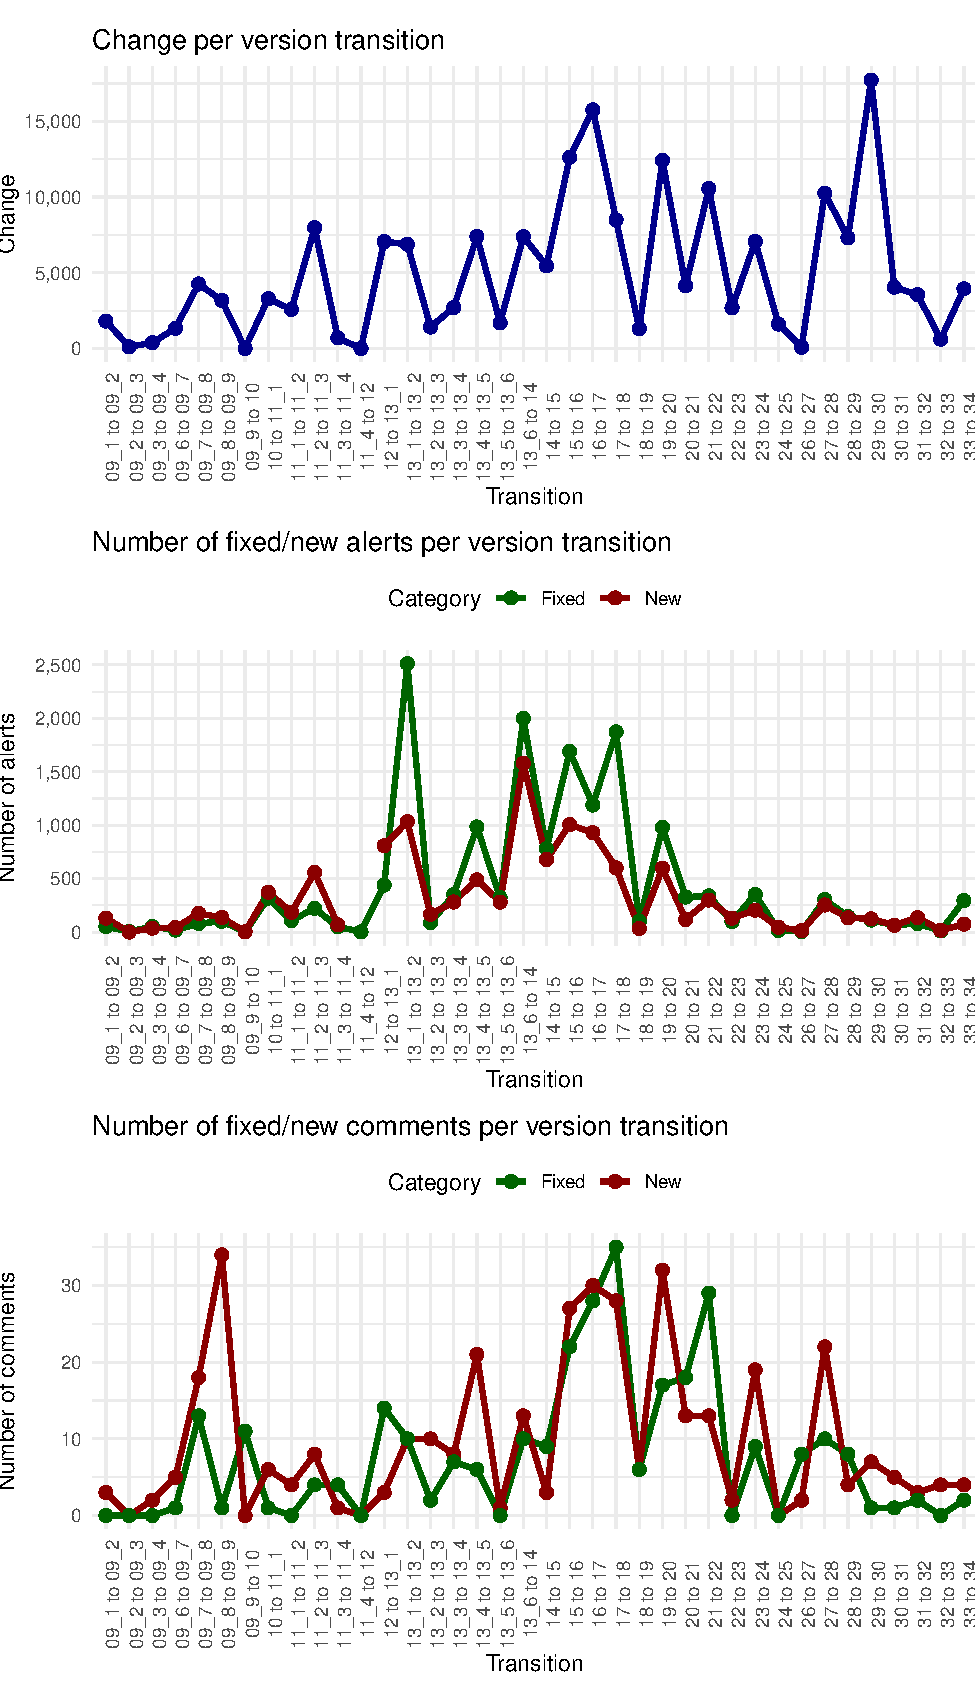
\includegraphics{report_files/figure-latex/unnamed-chunk-20-1.pdf}
\caption{\label{timeseries}Changes, alerts and comments}
\end{figure}

\normalsize

\newpage

We try to measure if there is a correlation between the amount of new
alerts and the amount of new comments.

Figure \ref{scatter_prop} shows the relation between the proportion of
new alerts and the proportion of new comments:

\[PropNewAlerts = \frac{NewAlerts}{NewAlerts + OldAlerts}\]

\[PropNewComments = \frac{NewComments}{NewComments + OldComments}\]

We can see that there is a positive correlation.

\small

\begin{figure}
\centering
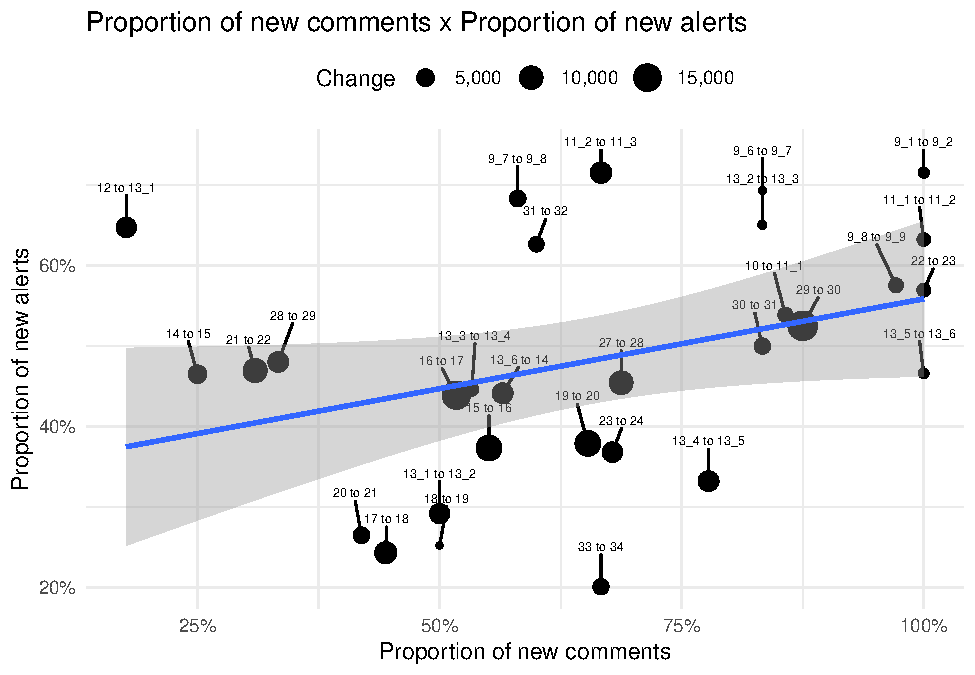
\includegraphics{report_files/figure-latex/unnamed-chunk-21-1.pdf}
\caption{\label{scatter_prop}Proportion of new alerts x Proportion of
new comments}
\end{figure}

\normalsize

In Figure \ref{scatter_diff} we correlate two metrics based on the
difference between the number of alerts and comments normalized by the
amount of change:

\[DiffNewAlerts = \frac{NewAlerts - OldAlerts}{Change}\]

\[DiffNewComments = \frac{NewComments - OldComments}{Change}\]

Where Change is calculated as in Equation \ref{eq_change}.

We can see that there is a positive correlation too.

\small

\begin{figure}
\centering
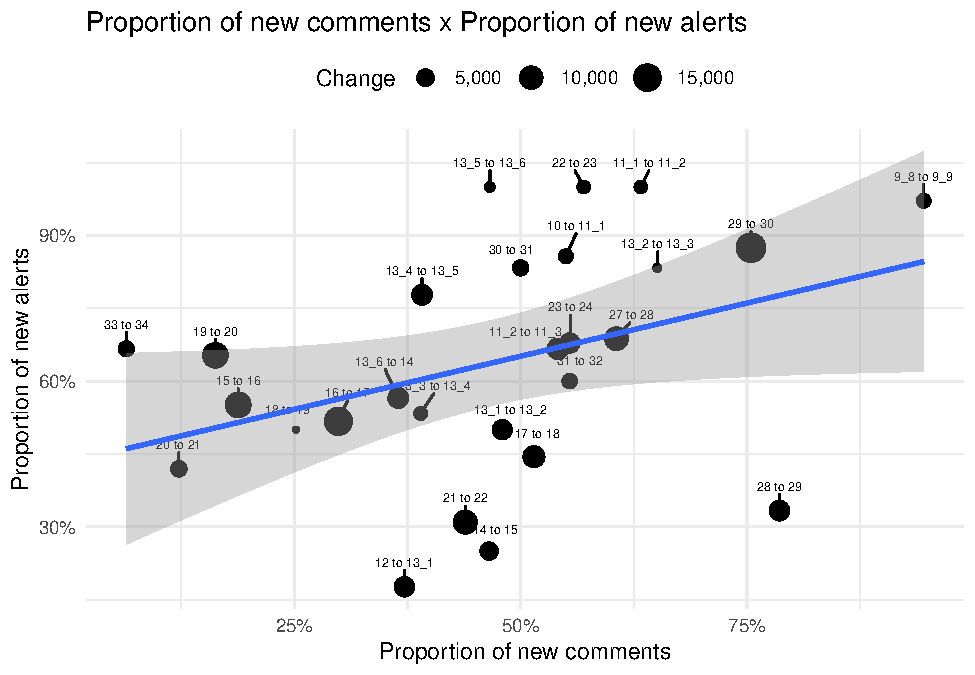
\includegraphics{report_files/figure-latex/unnamed-chunk-22-1.pdf}
\caption{\label{scatter_diff}Proportion of new alerts x Proportion of
new comments}
\end{figure}

\normalsize

It´s necessary to verify if the positive correlation that we found is
statistically significant. Table \ref{tab_reg} shows the results of
these regressions. In the form:

\[ NewAlertsProportion = \alpha + \beta NewCommentsProportions \]

and

\[ AlertsNormalizedDifferences = \alpha + \beta AlertsNormalizedDifferences \]

As we can see by the P-Value of the betas, we cannot reject the null
hypothesis in which there is no relation between comments and alerts.

\small

\begin{table}

\caption{\label{tab:unnamed-chunk-23}\label{tab_reg} Regression: alerts on comments}
\centering
\begin{tabular}[t]{l|l|l|l|l|l|l}
\hline
\multicolumn{1}{c|}{ } & \multicolumn{3}{c|}{Alerts Norm. Differences} & \multicolumn{3}{c}{New Alerts Proportions} \\
\cline{2-4} \cline{5-7}
Characteristic & Beta & 95\% CI & p-value & Beta & 95\% CI & p-value\\
\hline
(Intercept) & 0.34 & 0.17, 0.50 & <0.001 & -0.02 & -0.04, 0.00 & 0.045\\
\hline
New Comments Proportion & 0.22 & -0.01, 0.46 & 0.058 &  &  & \\
\hline
Comments Norm. Difference &  &  &  & 6.5 & -2.6, 16 & 0.16\\
\hline
\multicolumn{7}{l}{\textsuperscript{1} CI = Confidence Interval, CI = Confidence Interval}\\
\end{tabular}
\end{table}

\normalsize

In order to be able to reject the null hypothesis and accept that there
is a correlation between comments and alerts, we must run the same
procedures for more versions of the project and for more projects. We
can refine the way we select the comments, too. There are papers that
use more sofisticated schemes to identify SATD comments. These can be
our next steps.

\section{References}

\hypertarget{refs}{}
\leavevmode\hypertarget{ref-Potdar2014}{}%
Potdar, Aniket, and Emad Shihab. 2014. ``An exploratory study on
self-admitted technical debt.'' \emph{Proceedings - 30th International
Conference on Software Maintenance and Evolution, ICSME 2014}, 91--100.
\url{https://doi.org/10.1109/ICSME.2014.31}.

\leavevmode\hypertarget{ref-Sierra2019}{}%
Sierra, Giancarlo, Emad Shihab, and Yasutaka Kamei. 2019. ``A survey of
self-admitted technical debt.'' Elsevier Inc.
\url{https://doi.org/10.1016/j.jss.2019.02.056}.

\leavevmode\hypertarget{ref-Wehaibi2016}{}%
Wehaibi, Sultan. 2016. ``Satd-Patterns.''
\url{https://github.com/xsultan/satd-patterns}.

\end{document}
